\documentclass[a4paper, 12pt]{report}
\usepackage[latin1]{inputenc}
\usepackage[italian]{babel}
%\usepackage[T1]{fontenc}
\usepackage{graphicx}
\usepackage{float}
\usepackage[centertags]{amsmath}
\usepackage{amsfonts}
\usepackage{amssymb}
\usepackage{amsthm}
\usepackage{newlfont}
\usepackage{fancyhdr}
\usepackage{tesisty}

%-------------------------------
% DEFINIZIONE DEGLI ENVIRONMENT
%-------------------------------

\newtheorem{obs}{Osservazione}[section]
\newenvironment{oss}
    {\begin{obs}\begin{normalfont}}
    {\hfill $\square \!\!\!\!\checkmark$ \end{normalfont}\end{obs}}

\newtheorem{pro}{Problema}[chapter]
\newenvironment{prob}
    {\begin{pro}\begin{normalfont}}
    {\hfill $\spadesuit$ \end{normalfont}\end{pro}}

\newtheorem{teor}{Teorema}[section]
\newenvironment{teorema}
    {\begin{teor}\textit }
    {\hfill  \end{teor}}

\newtheorem{defn}{Definizione}[section]
\newenvironment{de}
    {\begin{defn}\begin{normalfont}}
    {\hfill $\clubsuit$ \end{normalfont}\end{defn}}

%-----------------------------
% CONFIGURAZIONE DELLA PAGINA
%-----------------------------

\hfuzz2pt % Don't bother to report over-full boxes if over-edge is < 2pt

\fancypagestyle{plain}{
\fancyhead{}\renewcommand{\headrulewidth}{0pt} } \pagestyle{fancy}
\renewcommand{\chaptermark}[1]{\markboth{\small CAP. \thechapter \textit{ #1}} {} }
\renewcommand{\sectionmark}[1]{\markright{\small  \thesection \textit{ #1}} {} }
\voffset=-20pt    % distanza tra il limite superiore del foglio e l'intestazione
\headsep=40pt     % distanza  l'intestazione ed il testo del corpo
\hoffset=0 pt     % misura equivalente al margine sinistro
\textheight=620pt % altezza del corpo del testo
\textwidth=435pt  % larghezza del corpo del testo
\footskip=40pt    % distanza tra il testo del corpo ed il pie' di pagina
\fancyhead{}      % cancella qualsiasi impostazione per l'intestazione
\fancyfoot{}      % cancella qualsiasi impostazione per il pie' di pagina
\headwidth=435pt  % larghezza del'intestazione e del pie' di pagina
\fancyhead[R]{\rightmark} \fancyfoot[L]{\leftmark}
\fancyfoot[R]{\thepage}
\renewcommand{\headrulewidth}{0.3pt}   % spessore della linea dell'intestazione
\renewcommand{\footrulewidth}{0.3pt}   % spessore della linea del pi�di pagina

\numberwithin{equation}{section}
\renewcommand{\theequation}{\thesection.\arabic{equation}}




%--------------------------
% MODIFICARE DA QUI IN POI
%--------------------------

\begin{document}

\dedicate{"C'\`e vero progresso solo quando i vantaggi di una nuova tecnologia diventano per tutti."\\Henry Ford}

\corso{INFORMATICA} \titoloTesi{La dinamica della rete Bitcoin: analisi empirica del vicinato di
un full-node} \anno{2018/2019}
\relatore{Dott. Francesco Pasquale}
 \autore{Marcello Politi}


\baselineskip=25pt

\intestazione

%------------------------------------------------
% INTRODUZIONE E RINGRAZIAMENTI (NON MODIFICARE)
%------------------------------------------------

\fancypagestyle{plain}{
\fancyhead{}\renewcommand{\headrulewidth}{0pt} } \pagestyle{fancy}
\renewcommand{\chaptermark}[1]{\markboth{\small Cap. \thechapter \textit{ #1}} {} }
\renewcommand{\sectionmark}[1]{\markright{\small  \S \thesection \textit{ #1}} {} }
\voffset=-20pt                         % distanza tra il limite superiore del foglio e l'intestazione
\headsep=40pt                          % distanza  l'intestazione ed il testo del corpo
\hoffset=0pt                           % misura equivalente al margine sinistro
\textheight=620pt                      % altezza del corpo del testo
\textwidth=435pt                       % larghezza del corpo del testo
\footskip=40pt                         % distanza tra il testo del corpo ed il pie' di pagina
\fancyhead{}                           % cancella qualsiasi impostazione per l'intestazione
\fancyfoot{}                           % cancella qualsiasi impostazione per il pie' di pagina
\headwidth=435pt                       % larghezza del'intestazione e del pie' di pagina
\fancyhead[R]{\rightmark} \fancyfoot[L]{\leftmark}
\fancyfoot[R]{\thepage}
\renewcommand{\headrulewidth}{0.3pt}   % spessore della linea dell'intestazione
\renewcommand{\footrulewidth}{0.3pt}   % spessore della linea del pi�di pagina

\pagenumbering{Roman} \tableofcontents
\newpage

\pagenumbering{arabic}

\fancyhead[R]{Introduzione} \fancyfoot[L]{Introduzione}
\fancyfoot[R]{\thepage}

\chapter*{Ringraziamenti}
Desidero ringraziare innanzitutto il relatore di questa tesi, il dott. Francesco Pasquale per la disponibilit\`a, l'attenzione e la gentilezza dimostrate durante la stesura del lavoro, ma sopratutto per il forte interesse che mi ha suscitato negli argomenti trattati durante le sue lezioni.\\
Inoltre vorrei ringraziare la mia famiglia, il mio punto di riferimento. In particolare mio padre che ha sempre creduto in me e con i suoi sacrifici mi ha permesso di raggiungere questo traguardo. Mia madre, che mi ha spronato e sostenuto in ogni momento, aiutandomi a trovare la grinta anche nelle circostanze pi\`u difficili. Mia sorella che, forse inconsapevolmente, mi trasmette continuamente la gioia e la spensieratezza e mi da la certezza di essermi sempre vicino.\\
Ai miei compagni di studio e non, e a chi mi \`e stato sempre a fianco.\\
Un sentito grazie a tutti!


\chapter*{Introduzione}
Sempre un numero pi\`u alto di servizi internet basano la loro infrastruttura di rete su un'architettura peer-to-peer (P2P), la quale permette una notevole resilienza, flessibilit\`a e rapidit\`a di adattamento.
Una delle sfide maggiori in questo tipo di reti \`e di garantire robustezza a prescindere da malfunzionamenti o attacchi esterni. La conoscenza della topologia della rete pu\`o essere la chiave sia di un miglioramente della performance del servizio che si poggia su di essa, sia di un attacco pi\`u mirato alla rete stessa, come ad esempio un \textit{denial of service}.
Inoltre l'anonimia potrebbe essere un obiettivo (e.g. \textit{TOR}) che pu\`o venire compromessa se un hacker \`e in grado di ricostruire i \textit{path} di comunicazione tra i nodi.\\
Il sistema di moneta digitale Bitcoin utilizza una rete P2P per trasmettere informazioni riguardanti le transazioni attraverso i partecipanti della stessa. Lo scambio di informazione segue il \textit{gossip protocol}: se un \textit{peer} riceve una nuova transazione, controlla che questa sia valida e la inotlra ai suoi vicini.
A  partire  dalla  sua  creazione nel 2009, Bitcoin ha conquistato un'attenzione sempre maggiore, complice  anche  il \textit{boom} osservato nel 2017, anno nel quale la valuta ha raggiunto una quotazione pari a circa 3.000.
L'obiettivo principale di Bitcoin \`e quello di garantire trasferimenti di denaro sicuro che non si basino sulla fiducia in terze parti (come ad esempio una banca), e questo  obiettivo  viene  raggiunto  distribuendo  una  copia  del  database  delle transazioni su ogni nodo del network, divenendo cosi la prima forma di pagamento \textit{trustless}.
Il  database, che prende il nome di \textit{blockchain}, tiene traccia di tutte le  transazioni  avvenute  nella  rete  dal  1 gennaio 2009. 

La validit\`a delle transazioni viene garantita da un meccanismo a firma digitale tramite chiave privata e pubblica, permettendo che solamente i reali possessori di una determinata somma possano spenderla.  Le transazioni vengono verificate, prima di essere immesse nella blockchain, da nodi speciali, denominati \textit{miners}. I \textit{miners} svolgono il duplice ruolo di verifica della transazioni e di emissione dei bitcoin. La \textit{blockchain} non  viene  aggiornata  in  \textit{real time}, ma viene aggiunto un gruppo di transazioni, chiamato blocco, in media ogni 10 minuti . Ogni volta che tale blocco viene aggiunto, il sistema emette una quantit\`a prestabilita di bitcoin , destinata al minatore che per primo \`e riuscito a verificarne la validit\`a.  Queste operazioni richiedono un notevole potere computazionale, perci\`o i minatori sono molti meno dei nodi totali della rete, ma il loro numero \`e comuqnue sufficiente a garantire la decentralizzazione della stessa. Un'ulteriore caratteristica di Bitcoin \`e che l'emissione dell'omonima valuta, denominata di seguito BTC, \`e limitata, e cresce nel tempo asintoticamente fino a raggiungere il limite prestabilito di 21 milioni di unit\`a.  In questo modo il valore non pu\`o essere manipolato tramite l'inflazione, come invece pu\`o accadere con le valute tradizionali. L'introduzione fin qui fatta \`e  volutamente  generica, poich\`e i dettagli tecnici verranno analizzati in seguito.
Si \`e scelto di suddividere il lavoro di questa tesi in tre parti. Nel primo capitolo si vedr\`a una spiegazione generale di quello che \`e il mondo Bitcoin, come tale tecnologia \`e nata e si \`e diffusa, e come un utente comune pu\`o usufruirne. Nella secondo capitolo invece verr\`a fatta un analisi pi\`u tecnica sulle principali innovazioni che hanno permesso di creare tutta l'infrastruttura che sta alla base del Bitcoin, mentre negli ultimi due capitoli mostreremo come con un applicativo, creato appositamente per questo fine, siamo riusciti a ricavare informazioni utili da dati reali riguardanti le connessioni di un \textit{full node} con i suoi \textit{peer}.



\section*{Scopo del lavoro}
In questo lavoro mi concentrer\`o a studiare la topologia della rete Bitcoin, o almeno come questa viene osservata da parte di un singolo \textit{full node}. Attraverso degli applicativi sviluppati appositamente per questo scopo, andremo a raccogliere dati che in seguito verranno elaborati allo scopo di estrarre informazioni utili riguardo le connessioni di un nodo verso altri \textit{peer} del network Bitcoin. Il risultato di questo lavoro dovr\`a essere visto comunque come un passo intermedio per il raggiungimenro di un obiettivo pi\`u ambizioso che punta ad inferire e a studiare le connessioni dell'intero network Bitcoin.





\fancyhf{} %elimina header/footer vecchi


\fancyhead[R]{\rightmark} \fancyhead[L]{\leftmark}
\fancyfoot[R]{\thepage}





%---------------------
% INCLUSIONE CAPITOLI
%---------------------

\chapter{Bitcoin}
\label{chap:fond}

\vspace*{1cm}

\section{Il mondo Bitcoin}
\label{sec:iniziare}
Bitcoin e' una collezione di concetti e tecnologie che costituiscono le basi per un ecosistema di una moneta digitale. L'unit\`a di conto di questa valuta e' il "bitcoin", scritto solitamente con la prima lettera minuscola o identificato dalla sigla \textbf{BTC } o \textbf{XBT}, e' usato per salvare o trasmettere la valuta tra i partecipanti della rete.\\
Per convenzione quindi se il termine Bitcoin \`e utilizzato con l'iniziale maiuscola si riferisce alla tecnologia e alla rete, mentre se minuscola (bitcoin) si riferisce alla valuta in s\`e.
Gli utenti possono fare con Bitcoin quello che \`e possibile fare con una qualsiasi moneta convenzionale, l'unica differenza \`e che il bitcoin \`e interamente virtuale, non esistono monete fisiche ma solamente transazioni che possono trasferire valuta da un mittente verso un destinatario.\\
Gli utenti di Bitcoin possiedono delle \textit{keys} (chiavi) \footnote{chiavi private e chiavi pubbliche: le transazioni di bitcoin, come verr\`a analizzato nel secondo capitolo, si
basano sulla tecnologia della crittografia asimmetrica (o crittografia a chiave pubblica/privata), in
particolare sul meccanismo delle firme digitali. } con le quali possono provare la loro propriet\`a di una somma di bitcoin all'interno del network. Con queste chiavi gli utenti possono firmare le varie transazioni per trasferire della valuta ad un nuovo proprietario.\\
Le chiavi sono solitamente memorizzate all'interno di un \textit{wallet} che \`e un applicazione per computer o smartphone che permette all'utente di effettuare operazioni complicate con molta facilit\`a, offrendo a quest'ultimo un' interfaccia \textit{user-friendly} \footnote{In informatica, di facile utilizzo anche per chi non \`e esperto.}. L'unico requisito richiesto per poter spendere bitcoin \`e la chiave con la quale l'utente pu\`o firmare le varie transazioni.\\
Bitcoin \`e un sistema distribuito peer-to-peer (\textbf{P2P}) \footnote{Architettura di rete informatica in cui i nodi sono tra loro paritetici, potendosi comportare sia da client che da server.}, come tale non esiste un server "centrale" o un punto di controllo.\\
I bitcoin vengono creati attraverso un processo chiamato \textit{mining}, un termine che ricalca metaforicamente l'attivit\`a di estrazione dell'oro da una miniera, il quale consiste in una competizione tra i partecipanti (i \textit{full-node} della rete) che attraverso il loro potere computazionale cercano di trovare una soluzione ad un problema matematico mentre processano le transazioni. In media ogni 10 minuti un \textit{miner} \`e in grado di trovare una soluzione a tale problema e a validare cos\`i delle transazioni, questo \textit{miner} verr\`a ricompensato con dei nuovi bitcoin. Il processo di \textit{mining} essenzialmente decentralizza il processo di emissione di moneta, e quindi elimina il bisogno di una banca centrale che si occupi di tale emissione.\\
La difficolt\`a del problema matematico che i \textit{miner} dovranno affrontare pu\`o essere modificato dinamicamente in modo da mantenere una media di un successo ogni 10 minuti, in questo modo anche se il numero di \textit{miner} dovesse mutare, la media dei successi resterebbe sempre invariata.\\
Il protocollo stabilisce inoltre che ogni 4 anni la percentuale di bitcoin che viene creata si dimezzi, e il numero totale di bitcoin che possono essere creati \`e fissato a 21 milioni, una volta raggiunta questa soglia non verrano pi\`u creati nuovi bitcoin. Possiamo quindi prevedere che il numero di bitcoin in circolazioni raggiunger\`a l'apice massimo (21 milioni) nel 2040. Grazie a questo i bitcoin non potranno essere inflazionati poich\`e non pu\`o essere "stampata" nuova moneta.\\
La moneta Bitcoin \`e la prima vera applicazione di questa invenzione \footnote{Bitcoin \`e solamente la prima di tante criptovalute, successivamente a Bitcoin furono create ad esempio \textit{Etherium, Ripple, Bitcoin Cash...}}, rappresenta il culmine di anni di ricerche nell'ambito della crittografia , dei sistemi distribuiti, e molteplici altre discipline, tuttavia "\textit{Non c'\`e nulla a cui lo
si possa paragonare}", dice il suo stesso ideatore Satoshi Nakamoto \footnote{Pseudonimo dell'inventore della criptovaluta Bitcoin }

\section{Cenni storici}
Bitcoin  \`e una \textit{criptovaluta} \footnote{Il vocabolo criptovaluta \`e l'italianizzazione dell'inglese cryptocurrency e si riferisce ad una rappresentazione digitale di valore basata sulla crittografia.} e un sistema di pagamento mondiale creato nel 2008 da un anonimo inventore noto con lo pseudonimo di Satoshi Nakamoto. Questa innovativa tecnologia fu presentata al mondo attraverso la pubblicazione del \textit{paper} (documento) \cite{nakamoto2008bitcoin}. Nakamoto ha cosi creato un sistema di denaro elettronico compltamente decentralizzato \cite{tschorsch2016bitcoin}, e l'innovazione principale che ha reso possibile ci\`o \`e stata l'elaborazione dell'algoritmo chiamato \textit{Proof-of-Work} che permette alla rete di arrivare ad un consenso generale sullo stato delle transazioni, grazie a tale algoritmo si \`e anche risolto il problema del \textit{double spend}, che consiste nel fatto di poter spendere la stessa valuta pi\`u di una sola volta.\\
Il network di bitcoin \`e iniziato nel 2009, grazie all' implementazione rilasciata da Nakamoto stesso, la quale poi negli anni ha visto pi\`u modifiche da parte di altri programmatori che con il loro contributo hanno reso sempre pi\`u efficiente il programma di Nakamoto. 
Nell'agosto 2010, una grave falla per la sicurezza venne trovata nel protocollo, a seguito della quale le
transazioni non venivano correttamente verificate prima di essere immesse nella blockchain, il che avrebbe potuto consentire ad un eventuale aggressore di generare una quantit\`a arbitraria di BTC. Tale falla venne sfruttata nel giro di pochi giorni, prima che venisse predisposta una patch correttiva, ma poi il "buco" venne chiuso e la situazione stabilizzata grazie a specifici interventi.
Negli anni successivi, il valore dei BTC \`e cresciuto sensibilmente, passando da semplici frazioni di dollaro a un ammontare di 10.092,20 dollari  \footnote{Data di rilevazione del prezzo: domenica 25 agosto 2019. (Fonte: blockchain.info)}
Questa tecnologia ha aperto le strade a nuovi studi nel campo del calcolo distribuito, dell'economia e dell'econometria.
\subsection{La storia del mining}
\label{sec:impostazione}
Il cosidetto \textit{\textbf{mining}} \`e il processo con il quale si registrano le transazioni nel libro mastro di Bitcoin, un registro che ogni nodo della rete Bitcoin possiede in cui sono salvate tutte le transazioni effettuate e validate fino a quel momento. Il libro delle passate transazioni \`e chiamato \textit{blockchain} ed \`e appunto una catena di blocchi. La \textit{blockchain} serve essenzialmente per avere una conferma all'interno della rete di avvenute transazioni. I nodi che si occupano di minare blocchi (\textit{miners}) devono inserire all'interno del blocco minato la \textit{proof-of-work} per far si che il blocco venga considerato valido. Questa \textit{proof-of-work} verr\`a verificata dagli altri nodi della rete non appena riceveranno il nuovo blocco minato. Intuitivamente la \textit{proof-of-work} ci d\`a la sicurezza che il nodo che ha minato il blocco ha realmente fatto del "lavoro", ha impiegato cio\`e il suo potere computazionale nella risoluzione di un problema matematico, e per questo viene ricompensato. Proprio come un comune lavoratore riceve lo stipendio per il lavoro svolto.
Minare un blocco \`e molto difficile (vedremo nei capitoli successivi i vari tecnicismi) quindi richiede un potere computazionale elevato.
La difficolt\`a del problema che i \textit{miners} devono risolvere pu\`o essere per\`o modificata dinamicamente. Nei primi anni di vita di Bitcoin, il mining era solamente un hobby per gli appassionati di criptovalute. Un semplice computer era l'unico hardware richiesto, ma nell'arco di 10 anni le cose sono cambiate drasticamente.\\
Nel 2009 i primi minatori utilizzavano CPU multi-core standard per produrre BTC a un ritmo di 50 btc per blocco. Un altro avvenimento fondamentale per la storia del mining accadde nell'ottobre 2010, un utente della community rilasci\`o il codice per il \textit{mining} bitcoin con GPU. Con l'aumentare delle difficolt\`a data dalle GPU che hanno aumentato l' \textit{hashrate} \footnote{Per hashrate si intende l'unit\`a di misura della potenza di elaborazione della rete Bitcoin. Per fini di sicurezza la rete Bitcoin deve eseguire delle operazioni matematiche intensive. Quando la rete raggiunge un hash rate di 10 Th/s, significa che pu\`o realizzare un trilione di calcoli al secondo. Fonte: https://bitcoin.org/it/glossario\#hash-rate}, aument\`o anche l'esigenza di hardware migliore e dedicato.\\
Il prezzo della criptovaluta insieme alla difficolt\`a del \textit{mining} continuavano a crescere, e con essi, i requisiti hardware necessari per guadagnare abbastanza fecero divenire le schede video obsolete per consentire agli utenti medi di fare soldi. Nel 2011 comparirono i primi dispositivi (\textit{FPGA}) facendo aumentare la possibilit\`a di guadagno dei \textit{miners}.
Il maggior vantaggio che comport\`o l'uso di questa tipologia di hardware era il minor consumo di energia. Consumava un terzo di energia rispetto alle \textit{GPU} per svolgere in modo efficace lo stesso compito.
Lo sviluppo degli \textit{FPGA} ha presto dato il via all'ingegnerizzazione dei sistemi \textit{ASIC}, che hanno il miglior rendimento tra potenza di calcolo e consumo di energia. Questo passaggio ha segnato il passaggio da un hobby ad una vera propria industria del \textit{mining}.

 





\section{Acquistare bitcoin}
Siamo ormai abituati ad effettuare pagamenti elettronici attraverso 
carte di credito, PayPal e conti bancari. Tutti questi meccanismi di pagamento appena citati hanno in comune il fatto di essere reversibili, con questo intendiamo che dopo che un utente ha inviato un certa somma di denaro, teoricamente pu\`o riappropriarsi del denaro spedito annullando la transazione. In Bitcoin questo \`e impossibile, le transazioni sono irreversibili, una volta che una transazione viene registrata all'interno della blockchain non c'\`e modo di tornare indietro. Come pu\`o o allora un nuovo utente della piattaforma Bitcoin entrare in possesso di bitcoin?\\
Poich\`e chi vende Bitcoin generalmente si fa pagare attraverso carta di credito (o simili), come fa allora questo venditore di bitcoin ad essere sicuro che l'acquirente non ritorni in possesso del denaro che ha usato per acquistare gli stessi (poich\`e come abbiamo detto un pagamento con carta di credito \`e reversibile)? Esistono alcuni metodi sicuri per i nuovi utenti che vogliono acquistare bitcoin: 
\begin{itemize}
\item Trovare un amico fidato che \`e gi\`a in possesso di bitcoin e comprarli direttamente da lui.
\item Usare un servizio come \textit{localbitcoins.com} per trovare un venditore di bitcoin nella tua area (solitamente questi sono venditori fidati).
\item Usare un bitcoin ATM della propria citt\`a. Questa non \`e nient'altro che una macchina che accetta contanti e invia direttamente bitcoin sul \textit{wallet} del tuo smartphone.
\item Utlizzare un sistema di cambio di valuta che accetti bitcoin associato alla propria banca.
\end{itemize}

\section{I wallet Bitcoin}
Un \textit{wallet bitcon} \`e un servizio che consente di interfacciarsi con il sistema Bitcoin. Esistono varie implementazioni di questi \textit{wallet} che si differenziano l'un l'altro in termini di qualit\`a, performance, sicurezza, privacy e affidabilit\`a. Esiste anche un \textit{wallet} conosciuto come "Satoshi Client" o "Bitcoin Core" che deriva dall'implementazione originale scritta da Satoshi Nakamoto.
I bitcoin non sono di fatto contenuti all'interno dei \textit{wallet} stessi, ma sono memorizzati in un registro aperto al pubblico, la \textit{blockchain}, sotto degli specifici indirizzi appartenenti ai diversi utenti. Gli indirizzi sono punti di ricezione e invio, e si presentano sotto forma di codici alfanumerici di 33 o 34 caratteri, generalmente inizianti per 1, come ad esempio \textit{1G1vTdCYjqb5gucmhNQH7yTBy9uPHC5Aht}, in modo da non contenere alcun
riferimento dell'utente utilizzatore, facendo di Bitcoin un sistema di pagamento pseudonimo. 
I \textit{wallet} custodiscono solamente le chiavi dell'utente, che gli permettono di spendere i bitcoin associati al preciso indirizzo che deriva dalla chiave pubblica che a sua volta deriva dalla chiave privata in oggetto. Quando si crea un nuovo \textit{wallet}, automaticamente vengono generate cento coppie di chiavi private e pubbliche (key-pool), per cui l'utente pu\`o usufruire di pi\`u indirizzi
diversi, per godere di maggiori livelli di privacy. 
Esistono diversi tipi di portafogli tra cui scegliere, a seconda dei livelli di praticit\`a, sicurezza e complessit\`a desiderata: 
\begin{itemize}
\item \textbf{Desktop Wallet}:  software \textit{wallet} da installare sul proprio computer che permette di memorizzare e custodire le chiavi private all'interno dell'hard disk. L'installazione di questi software, ce ne sono di vario tipo per diversi sistemi operativi, richiede generalmente il download dell'intera \textit{blockchain}. E' stato il primo tipo di \textit{wallet} creato.

\item \textbf{Mobile Wallet}: Questo \`e il pi\`u comune tipo di \textit{wallet} bitcoin. Pu\`o essere usato su smarthpone con sistemi operativi come Apple iOS e Android, questi 	\textit{wallet} sono spesso un ottima scelta per i nuovi utenti perch\`e sono semplici e intuitivi da utilizzare.

\item \textbf{Web Wallet}: I \textit{web wallet} sono acceduti tramite un web browser e salvano il \textit{wallet} di ogni utente su un server di un proprietario terzo.  Tipicamente i \textit{wallet} online sono offerti in via accessoria dagli exchange, piattaforme di compravendita di bitcoin in cambio di valute tradizionali. Considerando gli spiacevoli inconvenienti capitati ad alcuni di questi exchange in passato, probabilmente questo tipo di \textit{wallet} non \`e il pi\`u sicuro della lista, ma \`e sicuramente il pi\`u semplice e veloce da utilizzare, in quanto \`e possibile accedervi da qualsiasi dispositivo connesso a internet. 

\item \textbf{Hardware Wallet}:  Dispositivi creati appositamente per custodire le chiavi private degli indirizzi bitcoin e di altre criptovalute. Sono solitamente dei mini computer aventi un'unica funzione, quella di firmare digitalmente le transazioni con le chiavi private dell'utente. Questi si collegano al computer generalmente via
USB, e interagiscono con i software \textit{wallet} in tutta sicurezza anche se il computer risultasse compromesso. 

\item \textbf{Paper Wallet}: Le chiavi che controllano i bitcoin possono essere stampati su materiali come carta, metallo ecc... per avere un "salvataggio" a lungo termine. Ovviamente si tratta di una tecnologia non elevata ma permettono sicurezza. I salvataggi offline vengono spesso chiamati con il termine \textit{cold storage}.



\end{itemize}

 	

\section{Utilizzo nella vita quodituana}
Facciamo un esempio qui di come potrebbero essere utilizzati i bitcoin nella vita di tutti i giorni. Alice che possiede nel suo \textit{wallet} 0.10 BTC vuole effettuare una transazione per comperare una tazza di caff\`e nel negozio di Bob a Palo Alto, California. In questo caso il costo della tazza di caff\`e \`e di un dollaro e 15 oppure di 15 millibitcoin. Bob possiede nel suo negozio un sistema di pagamento automatico che genera uno speciale QR code contenente una richiesta di pagamento. A differenza di altri QR code che contengono solamente l'indirizzo di destinazione dei bitcoin, questo contiene in oltre, anche l'ammontare del pagamento, e una generica descrizione del tipo "Caff\`e di Bob". Questo rende pi\`u facile generare la transazione poich\`e Alice vedr\`a solamente un oggetto come quello mostrato in figura che dovr\`a scannerizzare con il proprio smartphone per generare una corretta transazione.
\begin{figure}[!h]
   
\includegraphics[width=0.375\textwidth]{imgs/QRcode.png}
   \caption{QR code per la richiesta di pagamento in BTC}
\end{figure}
Una volta generata la transazione di 0.0150 BTC verso il nagozio di Bob, Alice sempre attraverso il suo smartphone autorizza la transazione. Nel giro di pochi secondi Bob vedr\`a la transazione sul registro, e la transazione sar\`a quindi completata.
Possiamo esaminare la transazione effettuata una volta che \`e stata inclusa all'interno della blockchain usando un sito di \textit{explorer} (si veda~\cite{antonopoulos2017mastering} pp. 16-17).





\chapter{Come funziona il sistema Bitcoin?}
\label{chap:basi}

\vspace*{1cm}

\section{Crittografia}
\subsection{Introduzione}
\label{sec:sezioni}
Molte delle propriet\`a dei Bitcoin sono possibili grazie alla crittografia, con la quale possono essere generate chiavi digitali, indirizzi Bitcoin e firme digitali.
Bitcoin fa uso di una crittografia \textit{asimmetrica o a chiave pubblica}.
In questo tipo di crittografia ogni utente possiede una coppia di chiavi, una chiave privata e una chiave pubblica, utilizzate per criptare e decriptare delle informazioni che gli stessi si scambiano in un messaggio. Questo tipo di crittografia risulta molto pi\`u efficace rispetto alla crittografia simmetrica, in cui i corrispondenti cifrano e decifrano i dati scambiati utilizzando un'unica chiave segreta (ma in questo caso sorge il problema
di come scambiarsi in maniera sicura la chiave stessa).
La chiave privata \`e, appunto, tenuta segreta dal suo possessore, mentre chiave la pubblica pu\`o essere resa nota. La chiave pubblica \`e generata a partire dalla privata attraverso una funzione non iniettiva, ovvero dalla chiave pubblica \`e impossibile risalire alla chiave privata da cui deriva. Infine chiave privata e chiave pubblica hanno una specifica e diversa funzione: la chiave pubblica serve cifrare le informazioni da
inviare, informazioni che possono essere decifrate soltanto con la relativa chiave privata. 
Bitcoin si basa su una particolare crittografia asimmetrica chiamata \textit{moltiplicazione su curva ellittica} che offre un meccanismo per la creazione di una coppia di chiavi, una chiave pubblica che \`e usata per ricevere denaro, e una chiave privata usata invece per firmare le transazioni e spendere fondi.
La \textbf{chiave privata (k)} \`e semplicemente un numero casuale, poi da questa chiave usando appunto l' \textit{elliptic curve multiplication} si genera la chiave pubblica, dalla quale infine facendo uso di una \textit{funzione di hash} \footnote{Una funzione di hash h, \`e una funzione che mappa un messaggio arbitrariamente lungo in una stringa di lunghezza prefissata, cercando di far in modo che da questa stringa non si possa risalire al messaggio che l'ha generata.} \`e possibile generare l'\textit{address} (indirizzo Bitcoin) dello user.\\
Per creare la chiave privata si prendono 256 bit in modo casuale e si controlla che il numero risultante sia minore di un certo valore \textit{n} \footnote{In Bitcoin n=1,${1,158\times 10}^{77}$.} , in caso negativo si ripete l'esperimento rigenerando un altro numero casuale nello stesso modo.\\
La \textbf{chiave pubblica (K)} \`e calcolata dalla privata (k) usando la moltiplicazione su curva ellittica:
\begin{equation}
K=k\times G
\end{equation}
ove G \`e la costante di generazione di punti sulla curva. 

 
\subsection{Crittografia su curva ellittica}
\label{sec:sezioni}
La crittografia usata da Bitcoin si basa una particolare curva ellittica chiamata \textit{secp256k1} , definita dalla funzione:
\begin{equation}
{y}^{2} \mod p= ({x}^{3} +7) \mod p
\end{equation}\\
Notiamo che ci troviamo in un caso discreto, la curva sar\`a quindi descritta da solamente alcuni punti sugli assi cartesiani.\\
(Per semplificare il ragionamento possiamo pensare al caso reale, \textit{figura 2.1})
\begin{figure}[!hb]
   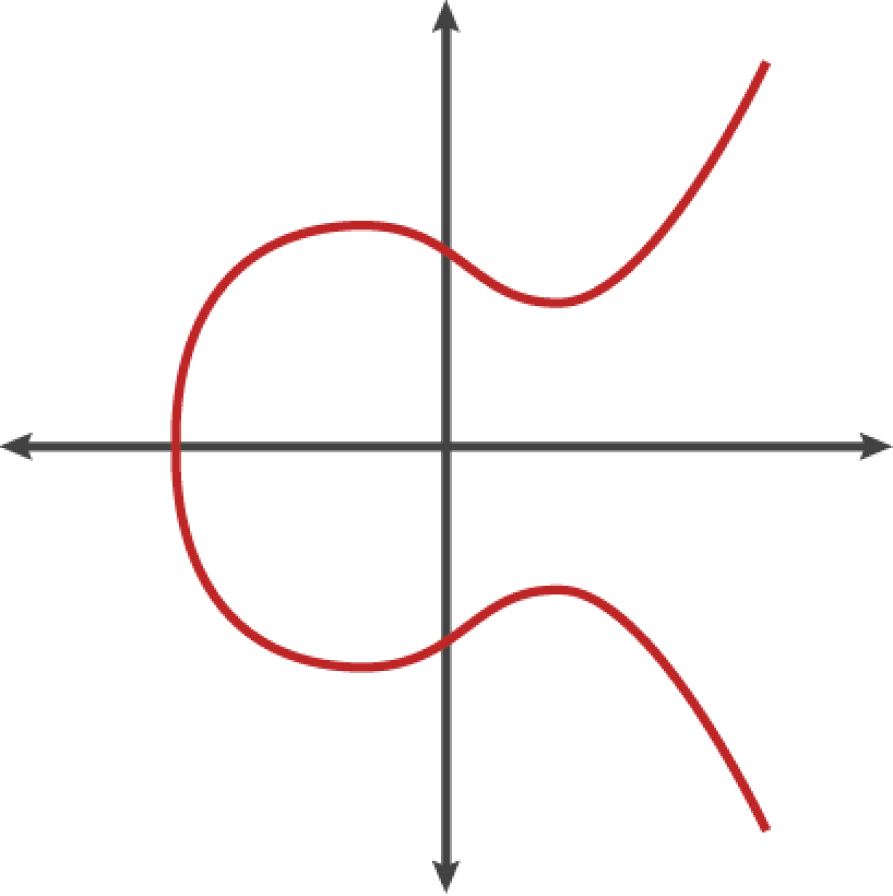
\includegraphics[width=0.375\textwidth]{imgs/mbc2_0402.png}
   \hfill
   \caption{Crittografia su curva ellittica: visualizzazione della curva ellittica con p=17, caso continuo}
   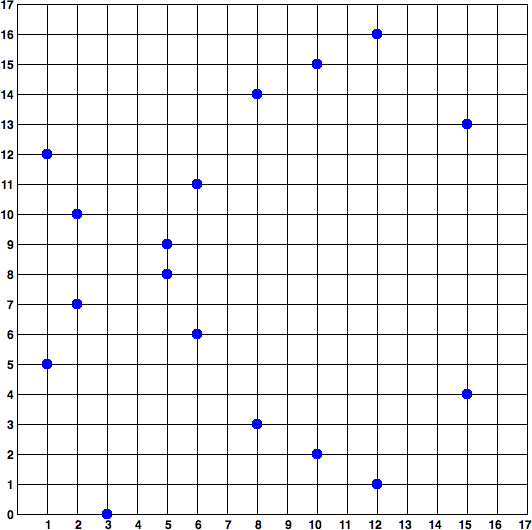
\includegraphics[width=0.375\textwidth]{imgs/mbc2_0403.png}
   \caption{Crittografia su curva ellittica: visualizzazione della curva ellittica con p=17, caso discreto}
\end{figure}\\Una propriet\`a fondamentale di questa curva \`e che dati due punti $P_1$ e $P_2$ $\in $ ad essa, allora anche $P_3=P_1+P_2 \ \in $ alla curva. 
Possiamo pensare alla moltiplicazione tra due punti della curva nel seguente modo:
se voglio moltiplicare un punto per un dato numero K, baster\`a sommare il punto a se stesso K volte, in questo modo risulta molto semplice ricavare la \textit{public key} dalla \textit{private key} attraverso la \textit{2.1.1}\\


\subsection{Indirizzi Bitcoin}
\label{sec:sezioni}
Un indirizzo Bitcoin  viene prodotto da una chiave pubblica, e consiste in una stringa che inizia con "1". Un indirizzo  pu\`o rappresentare il possessore di una coppia di chiavi (\textit{public/private key}) oppure qualcos'altro come uno script di pagamento.\\
Partendo dalla chiave pubblica ,vengono applicate due funzioni di hash,  uno \textit{SHA256} e poi \textit{RIPEMD160} sul risultato, ottenendo un numero a 160 bit (20 byte) che rappresenter\`a l' \textit{address} dell'utente:\\\\
$ A_{address}=RIPEMD160(SHA256(K))$\\\\
Gli indirizzi Bitcoin sono codificati in \textit{Base58Check} per proteggersi dagli errori umani. Questo formato \`e utilizzato perch\`e elimina i caratteri tra loro fraintendibili per l'occhio umano, inoltre sempre per prevenire un errore che pu\`o venire commesso da un utente la codifica \textit{Base58Check} crea un meccanismo di \textit{check} (controllo). Il \textit{checksum} \footnote{In telecomunicazioni e informatica il checksum  \`e una sequenza di bit che viene utilizzata per verificare l'integrit\`a di un dato o di un messaggio che pu\`o subire alterazioni durante la trasmissione sul canale di comunicazione.} sono 4 byte che vengono aggiunti alla fine dell'indirizzo, e derivano dalla funzione \textit{hash} di tutto quello che li precede, cosi possiamo sempre controllare la correttezza di un indirizzo.\\
Per convertire dei numeri (dati) in \textit{Base58Check} , per prima cosa creiamo un prefisso chiamato \textit{version-byte} che indica il tipo di dato, ad esempio per un indirizzo Bitcoin \`e 0 ( 0x00 in hex).\\
Poi si crea un checksum con un \textit{double SHA}:\\\\
$checksum=SHA256(SHA256(prefix+data))$\\\\
Dai 32 byte che risulteranno da questo procedimento prendo solo i primi 4.\\
Il risultato finale \`e quindi composto da: \textit{prefix,data,checksum}.
Il prefisso cambier\`a a seconda di cosa voglio codificare.
\begin{figure}[!h]
   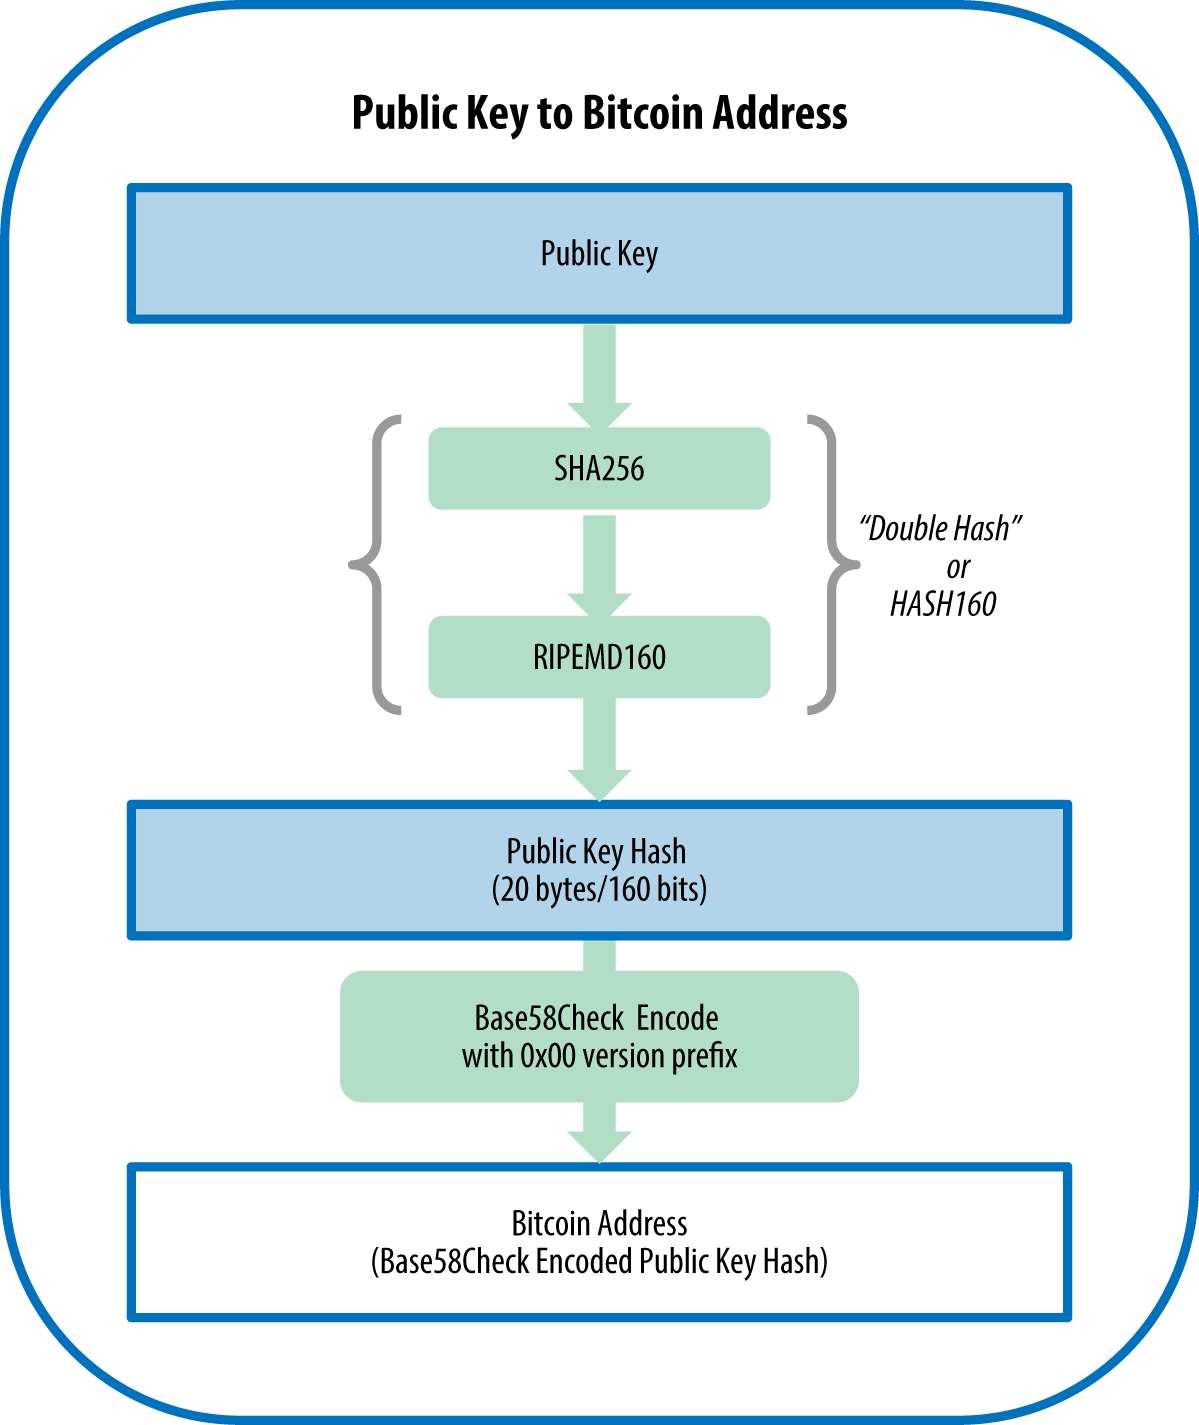
\includegraphics[width=0.675\textwidth]{imgs/address.png}
   \caption{Conversione da una chiave pubblica ad un indirizzo Bitcoin}
\end{figure}



\section{Le transazioni}
Le transazioni sono delle strutture dati che codificano il trasferimento di valori tra partecipanti del sistema Bitcoin, forniscono quindi agli utenti la possibilit\`a di spendere satoshis \textit{una sottounit\`a di bitcoin, che pu\`o essere paragonata ai centesimi di Euro}. Ogni transazione \`e composta da diversi elementi, che danno la possibilit\`a di poter svolgere a parimenti transazioni semplici e pi\`u complesse, a seconda delle esigenze.
Ogni nodo nel network Bitcoin dovrebbe essere in grado di trasmettere le transazioni nel network e farle minare in un blocco. 
Inoltre, ogni nodo dovrebbe essere in grado di controllare se:
\begin{itemize}
\item Il denaro speso nella transazione esiste realmente.
\item Il denaro \`e gi\`a stato utilizzato (problema del \textit{double spending}).
\item Chi spende il denaro ha effettivamente i diritti per poterlo fare.
\end{itemize}
L'idea generale delle transazioni nel network Bitcoin \`e quella di inviare degli Input che vanno a spendere degli Output. Ogni transazione ha quindi almeno un Input ed un Output. Ogni Input spende un Output precedente.
Ogni Output \`e quindi in una specie di sala d'attesa (e prende il nome di Output Non Speso, \textit{\textbf{UTXO}}), finch\`e un successivo Input non lo "spende".
Ogni transazione ha come prefisso il numero della versione, che ha lo scopo di indicare agli altri \textit{peer} ed ai \textit{miner} il corretto insieme di regole da usare per validarla. Questo da la possibilit\`a agli sviluppatori di poter creare nuove regole senza invalidare le transazioni precedenti.

\subsection{UTXO: output di transazione non spesi}
Gli output nelle transazioni sono pezzi indivisibili di bitcoin registrati nella \textit{blockchain}. Un \textit{full node} della rete traccia tutti gli output spendibili, conosciuti come \textbf{\textit{unspent transaction outputs UTXO}}. Ogni transazione rappresenta un cambiamento nell'insieme di UTXO. Quindi quando diciamo che il \textit{wallet} di uno user ha "ricevuto" bitcoin, intendiamo dire che il \textit{wallet} ha trovato un UTXO che pu\`o essere speso usando le proprie chiavi. Lo \textit{ user's bitcoin balance} \`e la somma degli UTXO che lo user pu\`o spendere.\\
Come un centesimo non pu\`o essere suddiviso, un Bitcoin non pu\`o essere suddiviso sotto l'ottavo decimale del \textit{satoshis}. Sebbene un output pu\`o avere un valore qualunque, una volta creato questo \`e indivisibile, gli output sono appunto \textbf{discreti} e \textbf{indivisibili}.
Ad esempio, se si possiede uno UTXO di 20 bitcoin e si vuole pagare 1 bitcoin, la transazione generata deve consumare tutti e 20 i bitcoin producendo 2 output, 1 BTC all'address desiderato, e gli altri 19 BTC al tuo proprio \textit{wallet} (come se fosse il resto).\\L'applicazione \textit{wallet} di uno user tipicamente seleziona tutti gli UTXO dello stesso per arrivare alla quantit\`a desiderata, per poter cosi effettuare il pagamento.\\C'\`e per\`o un'eccezione a questa catena di input e output, una speciale transazione chiamata \textbf{coinbase transaction}, che \`e la prima transazione contenuta in ogni blocco della blockchain. Questa transazione \`e posta li dal miner "vincente" e crea dei bitcoin spendibili dal miner stesso. La \textit{ coinbase transaction} non consuma UTXO, invece ha un input speciale chiamato \textit{coinbase}. Questo \`e come i Bitcoin vengono creati durante il processo di \textit{mining}.

\subsection{I fees di transazione}
La maggior parte delle transazioni includono \textit{fees}, delle ricompense in bitcoin per il lavoro svolto dai \textit{miner}. Analizziamo pi\`u in dettaglio come i fees vengono inclusi nelle transazioni. La maggior parte dei \textit{wallet} calcola e include \textit{fees} automaticamente.\\
Le \textit{transaction fees} (fees di transazione) servono come incentivo per includere (minare) una transazione nel prossimo blocco, possiamo vederle come una sorta di commissione.\\
Le \textit{transaction fees} sono calcolate in base alla dimensione della transazione in kilobytes, non in base al valore in BTC di essa, come si potrebbe pensare. I miner danno priorit\`a alle transazioni da includere nel blocco che sono in procinto di minare in base a vari criteri, tra questi c'\`e proprio la quantit\`a di 	\textit{fees} che ricaverebbero includendo una data transazione in tale blocco. Una transazione con sufficienti \textit{fees} \`e perci\`o pi\`u favorevole ad essere inclusa nel prossimo blocco, se invece i \textit{fees} sono troppo pochi la transazione pu\`o essere ritardata o addirittura neanche processata. Una transazione con \textit{fees} possimi allo zero rischia di non essere neanche propagata nel network.\\
Nel \textit{Bitcoin Core} (implementazione di riferimento di bitcoin) la politica dei \textit{fees} \`e settata dal \textbf{\textit{minerlayfee option}}. Attualmente il \textit{minerlayfee} \`e 0.00001 BTC per kilobyte.\\
Un algoritmo chiamato \textit{Fees Estimation Algorithm} calcola un ammontare di \textit{fees} appropriato affinch\`e i \textit{fees} offerti rendano la transazione competitiva all'interno del network. Si stima tramite questo algoritmo la quantit\`a necessaria di \textit{fees} che dia alla transazione un' alta probabilit\`a di essere inclusa da qui ad un certo numero di blocchi a venire. I servizi offrono di solito una alta, media, bassa probabilit\`a a seconda di della quantit\`a di \textit{fees} che si \`e disposti a pagare.\\


\subsection{Linguaggio di script delle transazioni}
L'\textit{engine} di validazione delle transazioni Bitcoin si basa su due tipologie di script, \textit{locking script} e \textit{unlocking script}.\\
Il \textit{locking script}  \`e posto su un output: specifica la condizione da soddisfare affinch\`e si possa spendere questo output in futuro. Il \textit{locking script} \`e chiamato anche \textit{scriptPubKey, witness script o cryptographic puzzle}.\\
L' \textit{unlocking script} risolve le condizioni poste su un output attraverso il \textit{locking script}, questa \`e parte dell'input di ogni transazione. Molto spesso gli \textit{unlocking script} contengono la firma digitale del \textit{wallet} dello user, prodotta dalla sua chiave privata.\\
L'algoritmo di firma digitale usato nei Bitcoin \`e l' \textit{Elliptic curve digital signature algorithm ECDSA}. La firma digitale ha tre scopi in Bitcoin:
\begin{enumerate}
\item La firma digitale d\`a prova della propriet\`a di una chiave privata, cio\`e del possessore dei fondi.
\item La prova dell' autorizzazione (a spendere) \`e innegabile.
\item La firma prova che la transazione non pu\`o e non deve essere modificata da nessuno dopo che \`e stata firmata.
\end{enumerate}
Ogni nodo di validazione dei Bitcoin, valider\`a le transazioni eseguendo il \textit{locking} e l' \textit{unlocking} script insieme. Il software di validazione copier\`a l' \textit{unlocking script}, prender\`a l' \textit{UTXO} referenziato dall'input, e copier\`a il  \textit{locking script} di questo \textit{UTXO}. Ora i due script saranno eseguiti in sequenza. Ci sar\`a la convalida se l' \textit{unlocking script } soddisfer\`a le condizioni del \textit{locking script}. Tutti gli input sono convalidati indipendentemente.
Il linguaggio di script della transazione Bitcoin \`e chiamato \textbf{Script}.
Questo contiene molti operatori, ma non contiene loop, solamente controlli condizionali. Il linguaggio quindi \textbf{\textit{non \`e Turing completo}}. Queste limitazioni permettono di non creare loop infiniti che possono essere usati come \textit{denial of service attack} contro la rete Bitcoin (Ricorda ogni transazione \`e validata da ogni full node).

\section{La rete Bitcoin }

\subsection{Architettura di rete peer-to-peer}
Il sistema Bitcoin \`e strutturato su un' architettura di rete \textit{peer-to-peer (\textbf{P2P})}. Con questo termine si indica che i computer che fanno parte della rete sono appunto "alla pari", non ci sono nodi "speciali", e perci\`o ogni nodo si assume la responsabilit\`a del funzionamento dei vari servizi di rete. Non c'\`e un server, non ci sono servizi centralizzati, e alcun tipo di gerarchia all' interno della rete. I nodi nella rete \textit{P2P} forniscono e allo stesso tempo consumano i servizi offerti dalla stessa. La caratteristica principale quindi di tale rete \`e il fatto di essere decentralizzata e aperta a chiunque. All'infuori di Bitcoin le applicazioni che hanno avuto pi\`u successo su questa architettura di rete sono \textit{Napster} e  \textit{BitTorrent}.\\
Bitcoin \`e nato per essere un sistema di moneta digitale su rete \textit{P2P}, e la decentralizzazione del controllo \`e il cuore dei principi di Bitcoin, e questa pu\`o essere raggiunta solamente sfruttando le caratteristiche di una tale rete.\\
Il termine \textit{Bitcoin Network} si riferisce all' insieme di nodi che stanno eseguendo il protocollo \textit{Bitcoin P2P}.

\subsection{I ruoli dei partecipanti della rete Bitcoin}
Sebbene i nodi in una rete \textit{P2P} siano alla pari, questi possono avere compiti differenti all'interno di essa. Un nodo Bitcoin implementa 4 diverse funzionalit\`a fondamentali:
\begin{itemize}
\item routing 
\item blockchain database
\item mining
\item servizi wallet
\end{itemize}
\begin{figure}[htb]
\begin{center}
   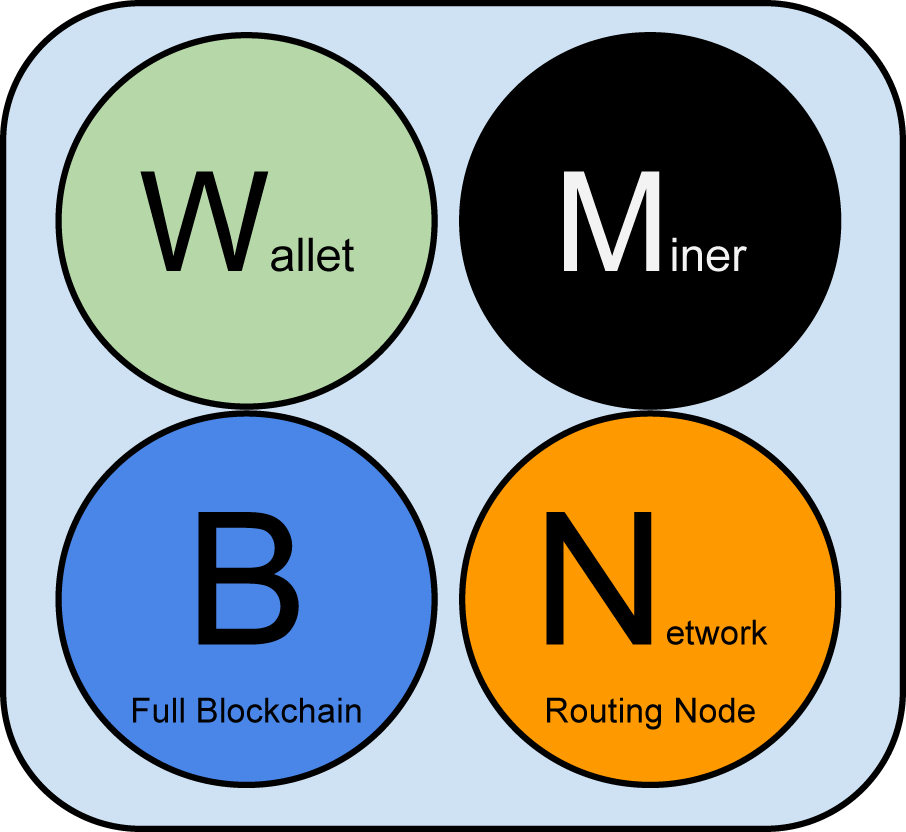
\includegraphics[width=0.355\textwidth]{imgs/4Funzioni.png}
   \caption{Un nodo della rete Bitcoin con tutte e quattro le funzionalit\`a: \textit{wallet, miner, full blockchain database e network routing}}
   \end{center}
   \hfill
\end{figure}
Tutti i nodi includono la funzioni di \textit{routing} per partecipare alla rete. Ogni nodo valida e propaga le transazioni e i blocchi sulla rete, inoltre scopre e mantiene connessioni verso altri \textit{peer}.\\
Alcuni nodi, chiamati \textit{full nodes}, mantengono anche una copia aggiornata della \textit{blockchain}. I \textit{full nodes} posso quindi verificare in autonomia le transazioni senza aver bisogno di referenze esterne. Alcuni nodi mantengono invece solamente una parte di tutta la \textit{blockchain}, e verificano le transazioni usando un metodo chiamato \textit{simplified payement verification , SPV}. Questi nodi sono chiamati nodi SPV o nodi \textit{lightweight}.\\
I nodi \textit{miner} competono per creare nuovi blocchi, utilizzando hardware dedicato alla risoluzione dell' algoritmo di \textit{Proof-of-work}. Alcuni nodi \textit{miner} sono anche \textit{full node}, cio\`e hanno una copia dell' intera \textit{blockchain}, mentre altri sono nodi \textit{lightweight} che partecipano a \textit{pool} di \textit{mining} dove soltanto il \textit{pool server} ha la funzionalit\`a di \textit{full node}.\\


\subsection{Come fa un nuovo partecipante a collegarsi alla rete Bitcoin?}
Quando un nuovo nodo si avvia, questo deve scoprire altri nodi all' interno della rete in modo da poter entrare a far parte dell'ecosistema Bitcoin. Per iniziare questo processo un nodo deve scoprire almeno un altro nodo all' interno della rete e connettersi con esso. La posizione geografica dei nodi \`e irrilevante, inoltre la topologia della rete Bitcoin non \`e geograficamente definita. Per questo, si pu\`o scegliere a caso qualsiasi nodo Bitcoin della rete.\\
Per connettersi a un \textit{peer} conosciuto, si stabilisce una connessione TCP, solitamente sulla porta 8333. Dopo aver stabilito la connessione, il nodo inizier\`a la fase di \textit{handshake} trasmettendo un messaggio denominato \textbf{\textit{version}} che contiene le seguenti informazioni:
\begin{itemize}
\item \textit{nVersion}:
La versione del protocollo Bitcoin P2P che il client "parla"
\item \textit{nLocalServices}:
Una lista di servizi locali supportati dal nodo
\item \textit{nTime}:
Il tempo corrente
\item \textit{addrYou}:
L'indirizzo IP del nodo remoto visualizzato da questo nodo
\item \textit{addrMe}:
L' indirizzo IP del nodo locale, come \`e stato scoperto dal nodo locale
\item \textit{subver}:
Mostra il tipo di software che sta girando su questo nodo
\item \textit{BestHeight}:
La lunghezza della blockchain 
\end{itemize}
Il messaggio di \textit{version} \`e sempre il primo messaggio inviato da ogni \textit{peer} agli altri \textit{peer}. Il \textit{peer} che riceve questo messaggio andr\`a a vedere se il nodo che sta provando a stabilire una connessione con lui \`e compatibile, facendo un check del campo \textit{nVersion}, in caso positivo risponder\`a con un messaggio di \textit{verack}.\\
\begin{figure}[!htb]
\begin{center}
   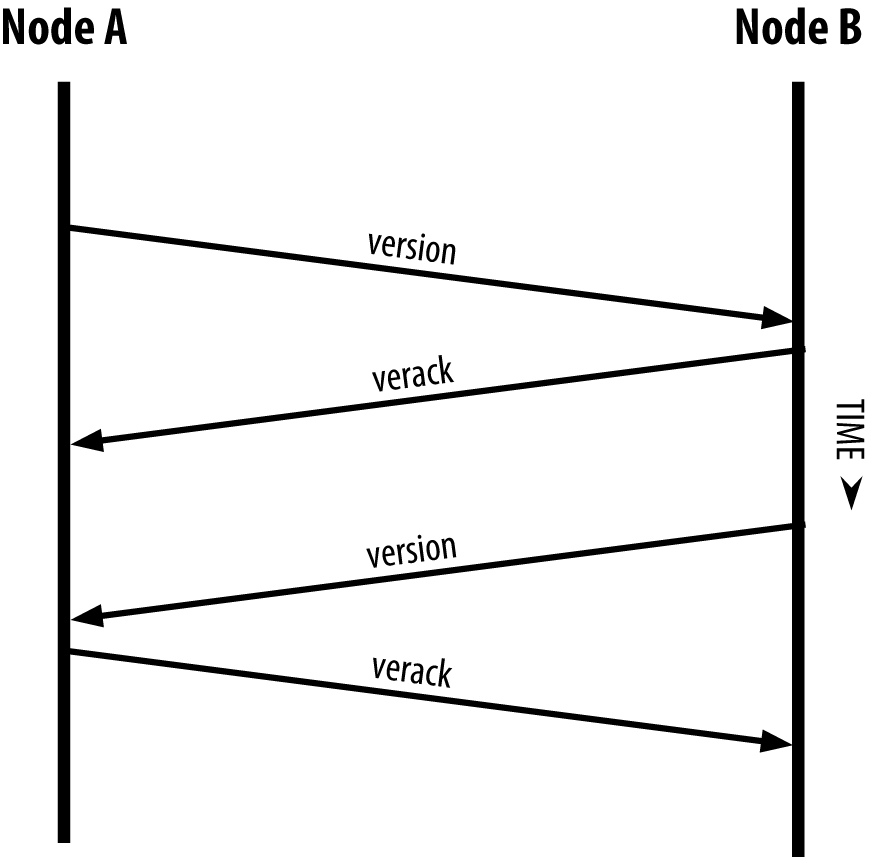
\includegraphics[width=0.455\textwidth]{imgs/connection.png}
   \caption{Handshake tra due peer della rete Bitcoin}
   \end{center}
   \hfill
\end{figure}\\\\
Come fa un nodo a trovare dei \textit{peer}?\\
Il primo metodo \`e facendo delle \textit{query DNS} a  dei \textit{DNS seeds} che sono server che forniscono indirizzi IP di nodi Bitcoin. Alcuni di questi \textit{DNS seeds} forniscono una lista statica di indirizzi di nodi Bitcoin stabili, altri invece ritornano un sottoinsieme random della lista degli indirizzi dei nodi Bitcoin collezionati da un \textit{crawler} della rete. Il \textit{Bitcoin Core} contiene al suo interno il nome di 5 differenti \textit{DNS seed}. Questi offrono un alto livello di affidabilit\`a per il processo iniziale di \textit{bootstrapping}.\\
Come alternativa, ad un nodo in fase di \textit{bootstrap} che non conosce nulla circa la rete, pu\`o essere fornito l' indirizzo IP di almeno un nodo che si trova nella rete, con il quale questo pu\`o stabilire una connessione e dal quale pu\`o ricevere maggiori informazioni riguardo la rete stessa. 
Una volta che una o pi\`u connessioni sono state stabilite, il nuovo nodo invier\`a un messaggio \textit{addr} ai suoi vicini contenente il proprio indirizzo IP. I vicini inoltreranno il messaggio \textit{addr} a loro volta ai loro vicini assicurandosi cos\`i che il nuovo nodo nodo sia ben connesso alla rete \footnote{Questo meccanismo di propagazione di messaggi all'interni di una rete viene chiamato \textit{gossip protocol}}. Il nuovo nodo in connessione pu\`o in aggiunta anche inviare un messaggio \textit{getaddr} ai suoi vicini, chiedendo loro di ritornare una lista di indirizzi IP di altri vicini.
\begin{figure}[!htb]
\begin{center}
   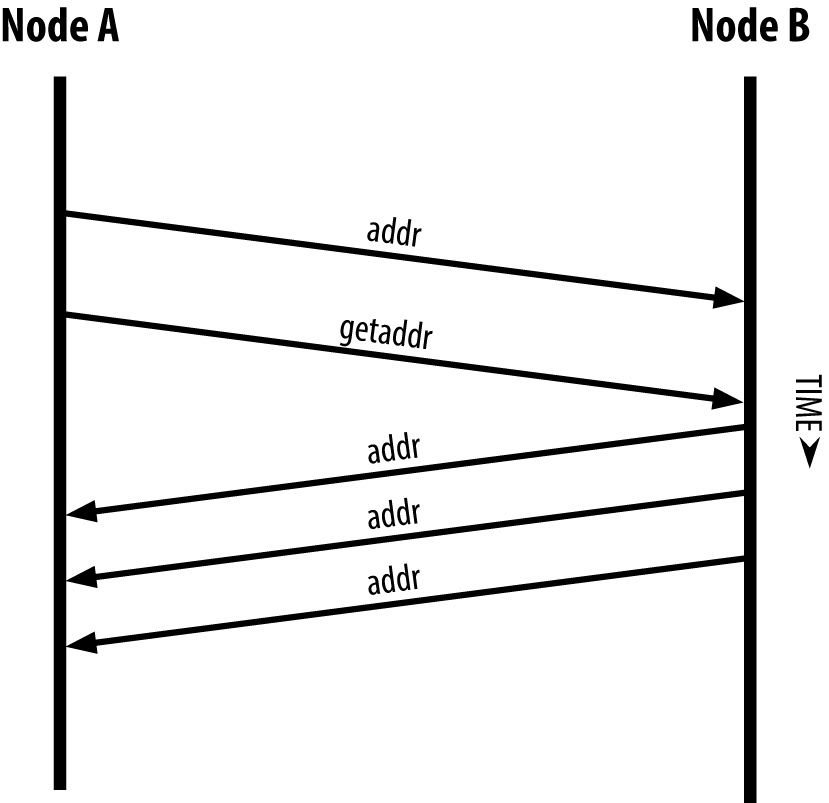
\includegraphics[width=0.455\textwidth]{imgs/addr.png}
   \caption{Propagazione di indirizzi Bitcoin}
   \end{center}
   \hfill
\end{figure}
Un nodo deve essere connesso ad alcuni \textit{peer} differenti in modo da poter stabilire dei path all' interno della rete Bitcoin. Questi path non sono del tutto affidabili, poich\`e i vicini di ogni nodo possono cambiare dinamicamente. Nella fase di \textit{bootstrap} c'\`e bisogno solamente di una connessione perch\`e questa fornir\`a informazioni su un altro nodo della rete che a sua volta far\`a in modo di collegarti a tutto il network. Dopo la fase di \textit{ bootstrap}, un nodo ricorder\`a un \textit{peer} con il quale \`e stato connesso, cos\`i ogni volta che verr\`a ravviato potr\`a collegarsi con questo senza passare nuovamente per la fase di \textit{bootstrap}.\\
Se non c'\`e traffico su una connessione, i nodi periodicamente si scambieranno dei messaggi per mantenere attiva la connessione, ma se questi smetteranno di comunicare per pi\`u di 90 minuti la connessione vierr\`a chiusa di default. Per questo la rete  \`e dinamica, pu\`o ingrandirsi o rimpicciolirsi senza un controllo centrale.

\subsection{Ricostruire la blockchain grazie al comando "Inventory"}
La prima cosa che deve fare un \textit{full node} che \`e appena entrato nella rete, \`e di provare a ricostruire tutta la \textit{blockchain}. Ogni nuovo nodo consce solo il primo blocco (\textit{genesis block} \footnote{Il genesis block pu\`o essere visualizzaro al link : https://www.blockchain.com/it/btc/block/000000000019d6689c085ae165831e934ff763ae46a2a6c172b3f1b60a8ce26f} ), il quale \`e incorporato all' interno del codice \textit{Bitcoin Core}. Il nuovo nodo deve quindi scaricare centinaia di migliaia di blocchi in modo da sincronizzarsi con tutta la rete.\\
Un nodo pu\`o vedere il messaggio \textit{version} mandatogli dai suoi \textit{peer}, conoscere cosi la quantit\`a di blocchi che loro possiedono, e compararli con la quantit\`a di blocchi che lui ha nella sua \textit{blockchain}.\\
Un \textit{peer} che ha una \textit{blockchain} pi\`u lunga di un altro, pu\`o identificare quali sono i blocchi che a quest' ultimo mancano per poterlo "raggiungere". Quindi identificher\`a i primi 500 blocchi da condividere e trasmetter\`a l' \textit{hash} di questi blocchi in un messaggio \textbf{\textit{inv}} (Inventory).\\
Il nodo che non possiede questi blocchi, cercher\`a di recuperarli usando una serie di messaggi \textit{getdata} richiedendo cosi i dati che compongono gli stessi.\\
Assumiamo per esempio, che un nodo abbia solamente il blocco iniziale. Questo ricever\`a un messaggio \textit{inv} dai \textit{ peer} contenente l' \textit{hash} dei prossimi 500 blocchi della catena. Il nodo inizier\`a a richiedere i blocchi a tutti i suoi vicini, mantenendo traccia di quanti blocchi sono "in transito" per ogni connessione \textit{peer}, stando attento a non superare il limite di una data costante: \textit{MAX\_BLOCKS\_IN\_TRANSIT\_PER\_PEER}. In questo modo, se esso necessita di molti blocchi, chieder\`a soltanto nuovi blocchi senza richiedere per due volte uno stesso blocco.


\section{La Blockchain}
La struttura dati della \textit{blockchain}, \`e una lista di blocchi ordinata, ognuno dei quali contiene delle transazioni. La \textit{blockchain} pu\`o essere registrata in un semplice database. I blocchi sono collegati l'un l'altro, ogni blocco fa riferimento a quello che lo precede. Spesso la \textit{blockchain} viene visualizzata come uno \textit{stack}, con questa visualizzazione viene spontaneo parlare di altezza della \textit{blockchain}, \textit{height}, termine con il quale si intende la distanza tra il primo e l'ultimo blocco dello \textit{stack}.\\
Ogni blocco \`e identificato da un \textit{hash}, generato usando l'algoritmo \textit{SHA256} sull' \textit{header} del blocco stesso. Ogni blocco quindi contiene all' interno del proprio \textit{header}, il campo \textit{previous block hash}, che non \`e altro che un puntatore al blocco genitore (blocco precedente). In altre parole ogni blocco contiene l' \textit{hash} del genitore all' interno del proprio \textit{header}.\\
Sebbene ogni blocco abbia un solo genitore, potrebbero avere per\`o temporaneamente pi\`u figli. Un blocco pu\`o avere pi\`u di un figlio quando si verifica una \textit{fork} nella \textit{blockchain}, cio\`e una situazione momentanea in cui due diversi blocchi sono stati scoperti quasi simultaneamente da \textit{miner} differenti. Ad ogni modo le situazioni di \textit{fork} vanno risolte facendo rimanere solamente uno di questi figli all'interno della catena.\\
Il campo \textit{previous block hash} \`e all' interno dell' \textit{header} dei blocchi, quindi ovviamente influenza l' \textit{hash} del blocco corrente. L'identit\`a del figlio cambia se cambia quella del genitore. Se in qualunque modo il genitore venisse modificato, verrebbe modificato anche il suo \textit{hash}. Il cambiamento dell' \textit{hash} del genitore necessita un cambiamento nel campo \textit{previous block hash} del figlio. Il cambiamento di questo campo a sua volta necessita che l' \textit{hash} del figlio cambi, cosi come l' \textit{hash} del nipote, e cosi via...\\
Questo effetto a cascata assicura che quando un blocco ne ha molti altri che lo succedono, questo non potr\`a essere modificato senza ricalcolare tutti gli \textit{hash} dei blocchi che lo succedono (cosa che richiederebbe una forza computazionale enorme!).\\
Per via della grande forza computazionale richiesta possiamo essere sicuri che una lunga catena di blocchi rende la storia della \textit{blockchain} immutabile, e questa \`e una delle caratteristiche principali della sicurezza della stessa.

\subsection{Il contenuto di un blocco della blockchain}
Un blocco \`e semplicemente una struttura dati che aggrega le transazioni al fine di includerle nel \textit{public ledger}, la \textit{blockchain}. Un blocco \`e composto da un \textit{header}, che contiene i metadati, seguito da una lunga lista di transazioni. L' \textit{header} dei blocchi \`e di 80 byte, in media ogni transazione \`e di 400 byte e sempre in media ogni blocco contiene circa 1900 transazioni.
L' \textit{header} dei blocchi consiste in tre insiemi di metadati. C'\`e un riferimento al blocco genitore che crea una connessione tra due blocchi successivi. Il secondo insieme di metadati consiste nei campi \textit{difficulty, timestamp, e nonce} che sono relative alla competizione dei \textit{miner} che vedremo pi\`u avanti. Infine il terzo insieme di metadati consiste nel \textit{merkle tree root}, una struttura dati utilizzata per recapitolare tutte le transazioni all' interno del blocco.
\begin{figure}[htb]
\begin{center}
   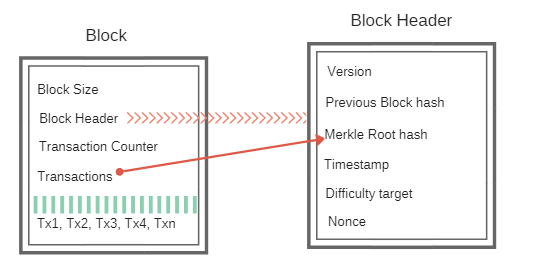
\includegraphics[width=0.755\textwidth]{imgs/block.png}
   \caption{Struttura dei blocchi }
   \end{center}
   \hfill
\end{figure}



\subsection{Identificazione dei blocchi attraverso header e height}
L'identificatore principale di un un blocco \`e il suo \textit{hash} crittografico, una firma digitale, creata applicando per due volte l'algoritmo \textit{SHA256} sull' \textit{header} del blocco stesso, i 32 byte risultanti sono chiamati \textit{block header hash}.\\
L' \textit{hash} identifica univocamente un blocco e pu\`o essere ricalcolato da ogni nodo semplicemente riapplicando lo \textit{SHA256} all' \textit{header} del blocco stesso. \\
Si noti che l' \textit{hash} di un blocco non \`e incluso all' interno della sua struttura dati , invece questo viene calcolato da ogni nodo non appena il blocco \`e propagato nel network.\\
Un secondo modo per identificare un blocco \`e guardando la sua posizione all' interno della \textit{blockchain}, la \textit{block height}.\\
Sebbene un blocco abbia sempre una specifica \textit{height}, il viceversa non \`e sempre vero. Due o pi\`u blocchi possono avere la stessa \textit{height}, quando sono in competizione per la stessa posizione all' interno della \textit{blockchain}, questo scenario \`e chiamato \textit{Blockchain Fork}. Neanche la \textit{block height} fa parte della struttura dati dei blocchi.
\paragraph*{Genesis Block} 
Il primo blocco nella blockchain \`e chiamato \textit{genesis block}, ed \`e stato creato nel 2009. Ogni nodo che entra a far parte del Bitcoin network ha una \textit{blockchain} che al suo interno contiene almeno questo blocco, poich\`e si trova all'interno dell'implementazione \textit{Bitcoin Core}. In questo modo ogni nodo ha un \textit{root} fidato dal quale pu\`o iniziare a costruire la propria catena di blocchi.

\subsection{Collegare i Blocchi nella Blockchain}
I Bitcoin \textit{full node} mantengono una copia locale della \textit{blockchain}, che viene costantemente aggiornata non appena arrivano nuovi blocchi. All' arrivo di un nuovo blocco, il \textit{full node} lo valider\`a e creer\`a un link per collegarlo alla \textit{blockchain} gi\`a esistente, per stabilire questo link il nodo andr\`a a vedere il campo \textit{previous block hash}, cosi da poter stabilire se il padre di questo nuovo blocco corrisponde all' ultimo blocco che lui ha in cima al suo \textit{stack} di blocchi.

\subsection{Merkle Trees}
Ogni blocco della \textit{blockchain} contiene un riepilogo di tutte le transazioni al suo interno tramite il \textit{merkle tree}. Il \textit{merkle tree}, conosciuto anche come \textit{binary hash tree}, \`e una struttura dati utilizzata per  verificare l'integrit\`a di un grande insieme di dati. I \textit{merkle trees} sono quindi alberi binari che contengono \textit{hash} crittografici.\\
Sono usati in Bitcoin per tenere traccia di tutte le transazioni in un blocco, producendo una firma digitale di un intero insieme di transazioni, e fornendo un meccanismo efficiente per verificare se una transazione \`e effettivamente inclusa in un blocco.\\
Il \textit{merkle tree} \`e costruito facendo ricorsivamente \textit{hash} di coppie di nodi fino a che non rimane solamente un nodo, chiamato \textit{root} o \textit{merkle root}. L'algoritmo di \textit{hash} crittografico usato \`e lo \textit{SHA256} applicato due volte.\\
Usando questa struttura, dati \textit{N} elementi all' interno del \textit{merkle tree}, possiamo verificare se uno specifico elemento cui siamo interessati \`e incluso nel \textit{tree} in al pi\`u $2\times\log_2{n}$ calcoli.\\
Il \textit{merkle tree} \`e costruito con un approccio \textit{bottom up}. Nel' esempio in figura \textit{2.8}, si parte da quattro transazioni (A,B,C,D) che formano le foglie dell'albero. Coppie consecutive di nodi sono riassunte nel nodo padre, concatenando i loro due \textit{hash} insieme. Il processo continua finch\`e non rimane solo un nodo in cima all' albero, il \textit{merkle root}. Perci\`o i 32 byte registrati nell' \textit{header} del blocco riassume tutte le transazioni che ne fanno parte.
\begin{figure}[htb]
\begin{center}
   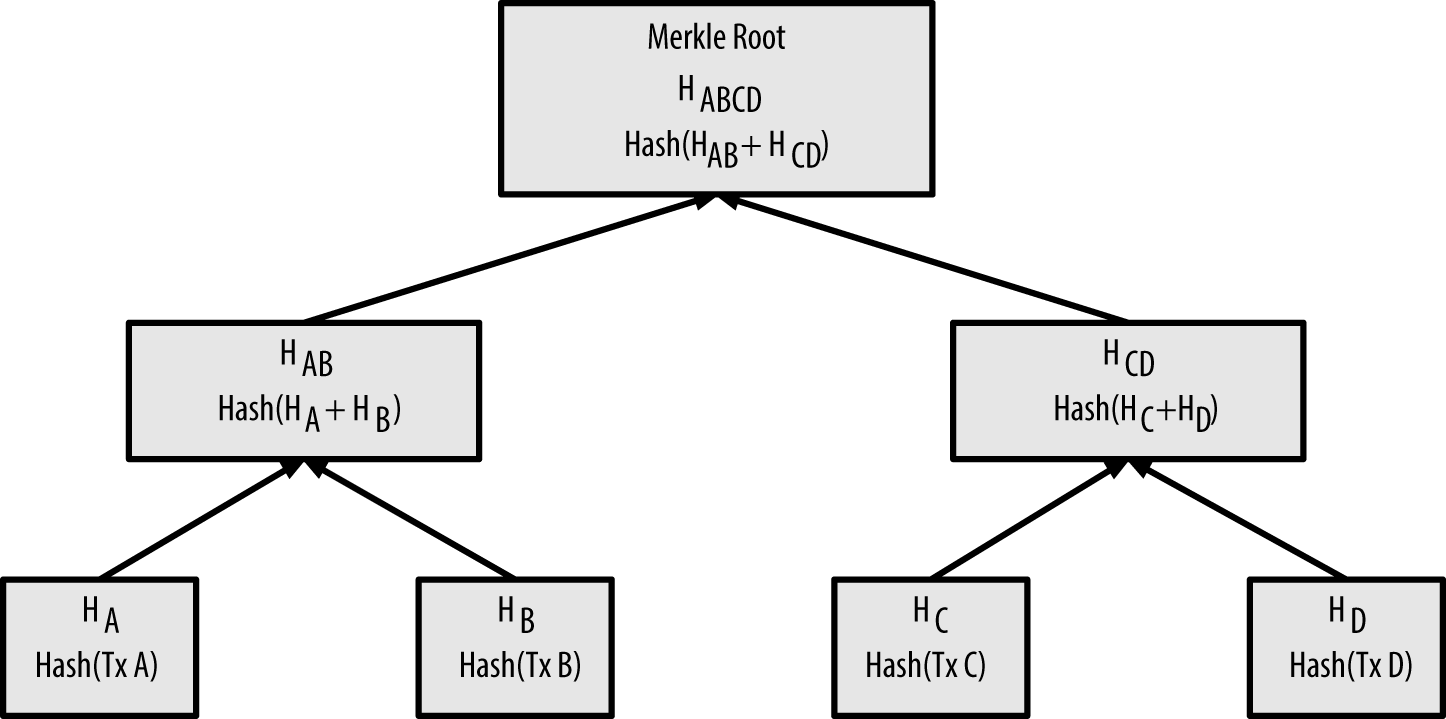
\includegraphics[width=0.755\textwidth]{imgs/merkleTree.png}
   \caption{calcolo dei nodi in un merkle root}
   \end{center}
   \hfill
\end{figure}
Poich\`e il \textit{merkle tree} \`e un albero binario, questo necessita di un numero pari di foglie. Se ci sono un numero dispari di transazioni, l' \textit{hash} dell'ultima transazione viene duplicato per creare un numero pari di foglie, l'albero che cosi viene a crearsi \`e conosciuto con il nome di \textit{balanced tree}.\\
In Bitcoin \`e comune avere migliaia di transazioni incluse in un blocco, quindi possiamo immaginare come le dimensioni dell'albero binario siano molto pi\`u grandi dell'esempio visto precedentemente.\\
Per provare che una transazione \`e davvero inclusa in un blocco, un nodo deve produrre solamente $\log_2{n}$ funzioni di \textit{hash}, costruendo cosi un \textit{authentication path} o \textit{markle path} che connetta quella specifica transazione al root dell'albero.\\
Nella figura seguente producendo un \textit{merkle path} vediamo come si pu\`o provare che la transazione \textit{K} \`e inclusa nel blocco. Il path consiste in quattro funzioni di \textit{hash} che e sono: $H_L,H_{IJ},H_{MNOP},H_{ABCDEFGH}$
\begin{figure}[htb]
\begin{center}
   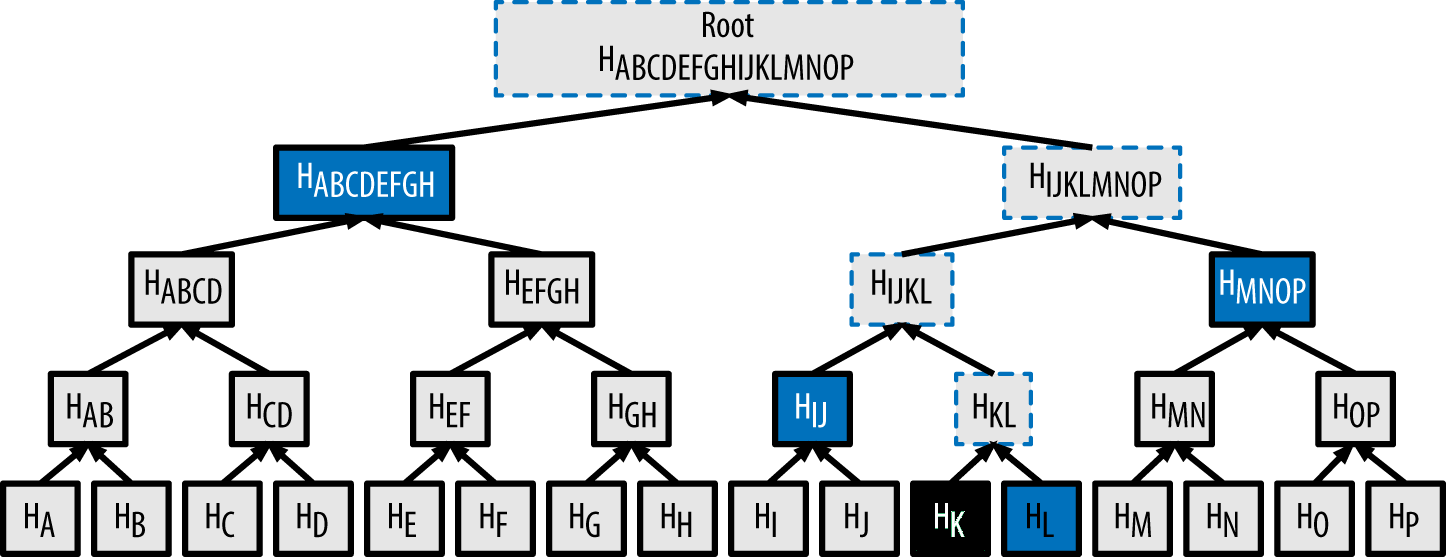
\includegraphics[width=0.755\textwidth]{imgs/merkleProof.png}
   \caption{Merkle path usato per provare l'inclusione dell' elemento K}
   \end{center}
   \hfill
\end{figure}
I nodi \textit{SPV} che non contengono una copia dell' intera \textit{blockchain}, usano i \textit{merkle path} per verificare le transazioni, senza dover fare il download di tutto il blocco.



\section{Mining per il consenso della rete}
\subsection{Introduzione}

L'obbiettivo principale del \textit{mining} non \`e la ricompensa o la generazione di nuovi \textit{coins}, ma il \textit{mining} \`e il meccanismo con il quale le transazioni vengono validate o
eliminate. Il \textit{mining} \`e ci\`o che rende Bitcoin un sistema sicuro e decentralizzato che \`e la base per una moneta digitale basata su rete \textit{P2P}.\\
Il \textit{mining} d\`a sicurezza al sistema Bitcoin e permette di creare moneta \textbf{senza un' autorit\`a centrale}. I \textit{miner} validano le nuove transazioni e le registrano nel \textit{public ledger} (libro mastro). Un nuovo blocco viene "minato" in media ogni 10 minuti. Le transazioni che diventano parte di un blocco e che sono quindi aggiunte alla \textit{blockchain} sono considerate confermate, questo permette al nuovo proprietario dei bitcoin di poter spendere i fondi di quella transazione.\\
I \textit{miner} ricevono due tipi di ricompense: ogni volta che viene minato un blocco vengono creati nuovi \textit{coins} che vengono assegnati al \textit{miner}, e inoltre questi ricevono i \textit{fees} da tutte le transazioni che fanno parte del blocco. Per guadagnare queste ricompense i \textit{miner} devono risolvere un complicato problema matematico basato su un algoritmo di \textit{hash} crittografico. La soluzione a tale problema, chiamato \textit{Proof of Work} \`e inclusa nel nuovo blocco minato, ed \`e prova del lavoro computazionale compiuto dal \textit{miner}.\\
Nuovi bitcoin sono quindi creati grazie al processo di \textit{mining}, in modo del tutto analogo a quando una banca stampa nuove banconote. La quantit\`a di bitcoin che vengono creati all'aggiunta di un nuovo blocco nella \textit{blockchain} diminuisce ogni 4 anni (ogni 210.000 blocchi). Facendo qualche conto si pu\`o notare che la ricompensa di bitcoin sar\`a diminuita esponenzialmente entro il 2140, data in cui non verranno pi\`u generati nuovi bitcoin oltre ai 20.999999998 milioni che saranno gi\`a in circolazione.\\
Abbiamo detto che i \textit{miner} ricevono anche come ricompensa i \textit{fees} da ogni transazione, oggi per\`o la ricompensa in \textit{fees} ricopre solamente il 5\% del guadagno di un \textit{miner}. Ad ogni modo poich\`e generazione di nuovi coins si abbasser\`a esponenzialmente, mentre il numero di transazioni per blocco aumenter\`a , arriver\`a un momento in cui la ricompensa in \textit{fees} sar\`a la parte dominante del guadagno dei  \textit{miner}.




\subsection{Consenso Decentralizzato}
La \textit{blockchain}, come visto nel capitolo precedente, \`e il libro mastro di tutte le transazioni, a cui ogni nodo della rete Bitcoin si affida.\\
Ma come possono tutti fidarsi di una singola \textit{verit\`a}, senza potersi e doversi fidare di nessun' altro all'interno della rete? I metodi di pagamento tradizionali dipendevano sempre da un' figura di autorit\`a centrale, Bitcoin non ha questa figura, ma in qualche modo ogni \textit{full node} ha una copia completa del libro mastro alla quale pu\`o affidarsi. Ogni nodo in qualche modo, attraverso lo scambio di informazioni sul network riesce ad arrivare alla stessa copia del libro mastro.\\
L'invenzione forse pi\`u importante introdotta da Satoshi Nakamoto \`e il meccanismo decentralizzato chiamato \textit{emergent consensus}. Il consenso \`e una caratteristica emergente dell' interazione asincrona di migliaia di nodi indipendenti che seguono delle semplici regole.\\
Il consenso decentralizzato dei Bitcoin emerge dall' interazione di quattro processi che si verificano indipendentemente sui nodi della rete: \
\begin{itemize}
\item Verifica indipendente di ogni transazione da parte di ogni \textit{full node}:\\
prima di propagare una transazione all'interno del network i \textit{full node} verificano che la transazione sia valida, in caso negativo questa sar\`a gi\`a scartata dal primo nodo.
\item Aggregazione indipendente di quelle transazioni nei nuovi blocchi fatta dai nodi \textit{miner}, attraverso la computazione della \textit{Proof of Work}.
\item Verifica indipendente dei nuovi blocchi , da ogni nodo e assemblamento in un catena.
\item Selezione indipendente da ogni nodo, della catena con pi\`u lunga.
\end{itemize}



\subsection{Aggregare Transazioni nei Blocchi}
Dopo aver validato le transazioni, un nodo Bitcoin le aggiunge nella \textit{memory/transaction pool}, dove queste attendono di essere incluse in un bloccco.\\
Descriviamo con un esempio ora il procedimento che compie un nodo \textit{miner} all'interno della rete.\\
Il nodo \textit{miner} di Gianni mantiene una copia locale della \textit{blockchain}. Allo stesso tempo Alice sta comprando una tazza di caff\`e, in questo momento la \textit{blockchain} di Gianni contiene 277,324 blocchi. Il nodo di Gianni rimane in ascolto per ricevere sempre nuove transazioni, prova a minare un nuovo blocco e inoltre controlla se qualche blocco \`e stato aggiunto da qualche altro \textit{miner} alla \textit{blockchain}.\\
Mentre il nodo di Gianni sta minando sfortunatamente viene annunciato il blocco 277,315 , cosi inizia subito la competizione per il blocco 277,316.\\
Durante i 10 minuti precedenti, mentre Gianni cercava di minare il blocco 277,315, stava allo stesso tempo collezionando transazioni da includere nel blocco. Adesso dovr\`a controllare che tra le transazioni che ha collezionato non ce ne sia qualcuna inclusa nel blocco 277,315, in tal caso dovr\`a eliminarla dalla \textit{transaction pool}.\\
Gianni costruisce immediatamente un blocco vuoto, candidato per la posizione 277,316, che viene appunto chiamato \textit{candidate block}, poich\`e il \textit{miner} ancora non ha trovato una soluzione all'algoritmo di \textit{Proof-of-Work}.

\subsection{La Transazione Coinbase}
La prima transazione in ogni blocco \`e speciale, viene chiamata \textit{coinbase transaction}. Questa transazione viene costruita dal nodo i Gianni come ricompensa degli sforzi fatti.\\
A differenza della transazioni comuni, la \textit{coinbase} non consuma \textit{UTXO} per i suoi input, invece ha solamente un input chiamato \textit{coinbase}.


\subsection{Minare il Blocco}
Adesso che il nodo di Gianni \`e stato costruito, \`e tempo di minare il blocco, trovando una soluzione al \textit{Proof of Work} che renda il blocco valido.\\
In termini semplici, minare \`e il processo in cui vengono eseguite tante funzioni di \textit{hash} ripetutamente, cambiando un solo parametro, fin tanto che il risultato dell'\textit{hash} non combaci con uno specifico target. Il risultato della funzione di \textit{hash} non pu\`o essere predeterminato, questa caratteristica fa in modo che l'unica maniera di produrre degli \textit{hash} che combacino con uno specifico target sia solamente provando e riprovando in modo del tutto casuale, modificando l'input.


\subsection{Algoritmo Proof-of-Work}
Un algoritmo di \textit{hash} prende in input un dato di lunghezza arbitrariamente lunga e produce un risultato di lunghezza fissa, la firma digitale dell'input. Per ogni specifico input, il risultato della funzione di \textit{hash} sar\`a sempre lo stesso. La caratteristica principale di un algoritmo di \textit{hash} crittografico \`e che \`e computazionalmente impossibile trovare due differenti input che producano la stessa firma (situazione nota come \textit{collisione}).\\
Con l'algoritmo di \textit{hash} usato in Bitcoin, \textit{SHA256}, l'output ha una lunghezza fissa di 256 bit. Vediamo degli esempi in cui ad una particolare stringa viene aggiunto un numero (\textit{nonce}) che cambia continuamente e alla quale applichiamo l'\textit{l'hash} crittografico:\\
Io sono Marcello Politi0 := a80a81401765c8eddee25df36728d732...\\
Io sono Marcello Politi1 := f7bc9a6304a4647bb41241a677b5345f...\\
Io sono Marcello Politi2 := ea758a8134b115298a1583ffb80ae629...\\
Io sono Marcello Politi3 := bfa9779618ff072c903d773de30c99bd...\\
Io sono Marcello Politi4 := bce8564de9a83c18c31944a66bde992f...\\
Io sono Marcello Politi5 := eb362c3cf3479be0a97a20163589038e...\\
Io sono Marcello Politi6 := 4a2fd48e3be420d0d28e202360cfbaba...\\
Io sono Marcello Politi7 := 790b5a1349a5f2b909bf74d0d166b17a...\\
Io sono Marcello Politi8 := 702c45e5b15aa54b625d68dd947f1597...\\
Io sono Marcello Politi9 := 7007cf7dd40f5e933cd89fff5b791ff0...\\
Io sono Marcello Politi10 := c2f38c81992f4614206a21537bd634a...\\
Io sono Marcello Politi11 := 7045da6ed8a914690f087690e1e8d66...\\
Io sono Marcello Politi12 := 60f01db30c1a0d4cbce2b4b22e88b9b...\\
Io sono Marcello Politi13 := 0ebc56d59a34f5082aaef3d66b37a66...\\
Si pu\`o notare che cambiando soltanto il \textit{nonce} finale, l'\textit{hash} della stringa cambia totalmente.\\
Per complicare un p\`o il tutto, fissiamo un target: troviamo quindi una stringa che produca un \textit{hash} esadecimale che inizi con la cifra 0. Fortunatamente non \`e difficile, se vediamo il tredicesimo tentativo rispetta i nostri criteri. In termini di probabilit\`a, se gli output della funzione di \textit{hash} sono equamente distribuiti, ci aspettiamo di trovare uno 0 in prima posizione una volta ogni 16 tentativi in media.\\
Notiamo anche che l'obbiettivo da noi posto equivale a trovare un \textit{hash} inferiore a:\\
0x1000000000000000000000000000000000000000000000000000000000000000\\
che \`e appunto il nostro \textit{target}. Se abbassassimo il target il nostro obbiettivo diventerebbe sempre pi\`u difficile.\\
Per capire meglio facciamo una semplice analogia. Immaginiamo un gioco in cui i giocatori tirano due dadi, e la somma di questi deve essere inferiore ad un certo target. Inizialmente il target \`e 12, quindi a meno che non si lanci un doppio 6, vinciamo sicuramente, quindi sembra in questo caso che il gioco sia molto semplice. Andando avanti per un paio di turni il target si abbassa a 5. Adesso notiamo che pi\`u del doppio dei lanci che possiamo fare risulter\`a fuori target, il gioco \`e diventato molto pi\`u difficile da vincere. Nel caso i target sia 2 (il minimo possibile) abbiamo solo un lancio che ci far\`a vincere, e in questo caso ci aspettiamo che di tirare un doppio 1 una volta ogni 36 lanci. In questo modo possiamo fare una stima dei lanci che abbiamo bisogno di fare per vincere, e questo ci da una prova che abbiamo fatto diversi tentativi prima di vincere, lo stesso vale quindi per i \textit{miner}, il fatto che trovino un \textit{hash} che rispetti il target \`e un \textit{proof} (prova) \textit{of work} (del lavoro fatto).\\
Nell' esempio mostrato precedentemente il \textit{nonce} vincente era il numero 13, e questo risultato pu\`o essere confermato da qualunque nodo indipendentemente. Tutti possono aggiungere il suffisso "13" alla frase "Io sono Marcello Politi" ed eseguirne l'\textit{hash} per vedere che quello che ne viene fuori sia un numero minore del target. Conoscendo il target ognuno pu\`o fare una stima della difficolt\`a di risolvere la \textit{Proof of Work} e conoscere quindi quanto lavoro ci vuole per trovare il \textit{nonce}.\\
Abbiamo gi\`a visto come un \textit{miner} costruisce un \textit{candidate block} pieno di transazioni. Successivamente il \textit{miner} calcola l' \textit{hash} dell'\textit{header} del blocco e verifica che sia pi\`u piccolo del target, se non lo \`e il \textit{miner} modificher\`a il \textit{nonce} e prover\`a nuovamente.



\chapter{Analisi delle connessioni di un singolo nodo}



\vspace*{1cm}

\section{Motivazioni}
Abbiamo visto nei capitoli precedenti come pu\`o essere utilizzata la tecnologia introdotta da Satoshi Nakamoto, e analizzato anche al livello pi\`u tecnico le parti fondamentali che costituiscono l'ecosistema Bitcoin.\\
In questo, e nel successivo capitolo voglio focalizzarmi sulla topologia della rete \textit{peer-to-peer} sulla quale si poggia Bitcoin.
Si \`e gi\`a accennato il fatto che la topologia di tale rete \`e deliberatamente tenuta nascosta, ma quali sono le motivazione principali del perch\`e debba essere segreta?
La conoscenza della topologia della rete non deve essere per forza considerata una minaccia o una vulnerabilit\`a, sebbene potrebbe comunque essere utilizzata in modo inappropiato da parte di hacker che potrebbero creare attacchi che hanno come bersaglio la rete stessa o rendere note le identit\`a degli \textit{user}, sappiamo bene che l'anonaminit\`a \`e una delle caratteristiche pi\`u apprezzate della tecnologia Bitcoin.
Un esempio di attacchi di questa tipo \`e l' \textit{eclipse attack}, basato su un network decentralizzato in cui chi attacca cerca di isolare uno specifico \textit{user} anzich\`e attaccare l'intera rete, e ovviamente conoscendo la topologia della stessa risulterebbe molto pi\`u facile identificare quali siano i nodi con meno connessioni e quindi pi\`u isolati.
Uno studio sulla topologia della rete potrebbe comunque rivelare delle caratteristiche interessanti riguardanti la stessa, si potrebbe vedere in che misura la rete sia veramente decentralizzata identificando \textit{supernodi}, \textit{nodi ponte}, \textit{potenziali punti di rottura,} ecc.. 
Lo studio della topologia della rete di Bitcoin \`e stato argomento di studio da parte di vari gruppi di ricerca, ognuno dei quali ha affrontato il problema di inferire le connessioni del network in maniera e con tecniche differenti.
La tecnica mostrata nel paper \cite{delgado2018txprobe} si basa fortemente sul monitoraggio delle \textit{pool} delle transazioni orfane e su come queste vengano propagate all'interno del network Bitcoin. Un approccio differente \`e invece quello descritto in \cite{miller2015discovering} dove le connessioni tra i nodi vengono identificate attraverso l'analisi dei \textit{timestamp} i quali vengono aggiornati continuamente quando i nodi della rete si scambiano messaggi. Infine vorrei citare il \cite{neudecker2016timing} nel quale viene mostrato come inferire la topologia della rete Bitcoin facendo osservazioni e comparazioni tra le informazioni riguardo al \textit{delay} di propagazione della rete Bitcoin e il \textit{delay} di propagazione di un modello matematico scelto come confronto. \\
In questa tesi avremo un obiettivo meno ambizioso, andremo ad analizzare coma cambia la rete dal punto di vista di un singolo nodo. Per questo esperimento si \`e installato un \textit{full node} che monitoreremo periodicamente per ricavare dei dati circa lo stato delle sue connessioni con altri \textit{peers}, si andr\`a poi a fare un analisi dei dati cosi raccolti, attraverso un programma scritto in python che evidenzier\`a varie caratteristiche derivate dall'elaborazione di questi dati come ad esempio la percentuale dei nodi che rimangono connessi dall'inizio alla fine della monitorizzazione, la probabilit\`a in media che una connessione "crolli", metter\`a in risalto inoltre quei nodi che sono rimasti connessi per pi\`u tempo poich\`e potrebbero essere nodi stabili della rete, sar\`a mostrato con un grafico a barre per ogni \textit{peer} (identificato dall'indirizzo IP) la percentuale di tempo che \`e rimasto in connessione con il nostro \textit{full node} e vederemo se l'analisi di differenti monitorizzazioni produrranno risultati simili.




\section{Descrizione dell'applicativo}
L'applicativo consiste nel richiamo periodico del comando \textit{bitcoin-cli getpeerinfo} da parte di un \textit{full node} in nostro possesso. Questo comando ritorna alcune informazioni riguardanti le connessioni del nodo verso altri nodi della rete, possiamo vedere un esempio nella figura \textit{3.1}.
\begin{figure}[H]
\begin{center}
   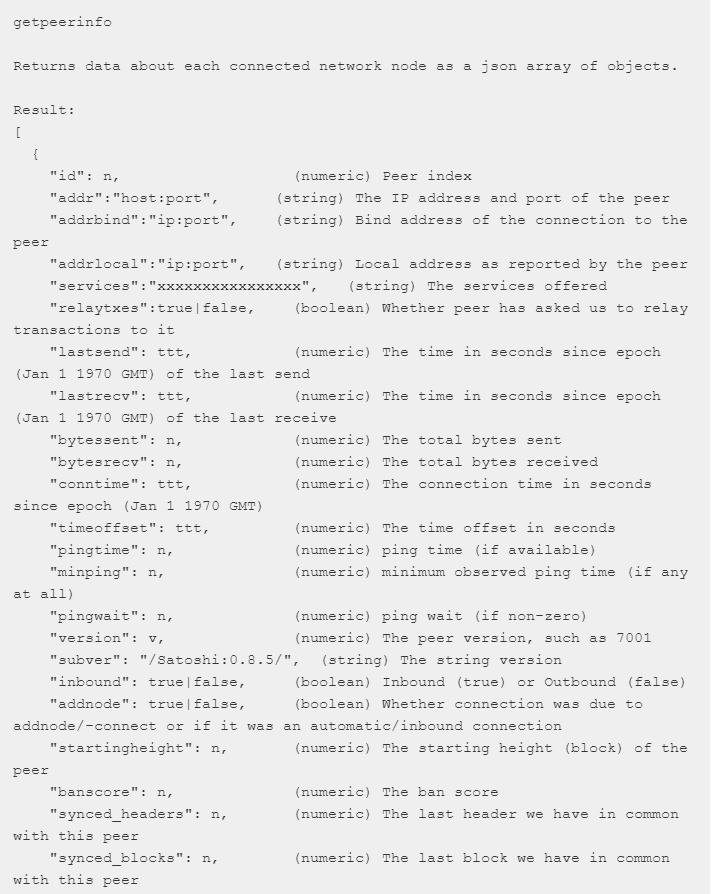
\includegraphics[width=0.555\textwidth]{imgs/getpeerinfo.png}
   \caption{https://bitcoincore.org/en/doc/0.16.0/rpc/network/getpeerinfo/}
   \end{center}
   \hfill
\end{figure}
Lanciando pi\`u volte il comando appena descritto potremmo ricavare dati utili da elaborare con lo scopo di capire il comportamento del nostro nodo e i suoi vicini all'interno del network.\\
L'applicativo consiste in due programmi scritti in python, \textit{raccolta\_dati\_csv.py} e \textit{analisi\_dati\_csv.py}.
Il primo serve appunto per raccogliere informazioni circa il nostro \textit{full node}, quando viene richiamato questo richiede un parametro, \textit{param1}, che indica il nome del file che il programma andr\`a a creare per salvare i dati raccolti (si veda figura \textit{3.2}).
\begin{figure}[htb]
\begin{center}
   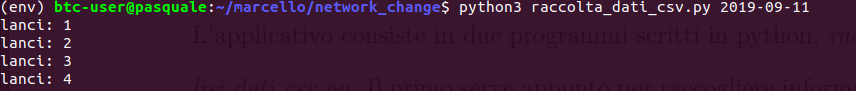
\includegraphics[width=0.755\textwidth]{imgs/raccolta_dati_csv.png}
   \caption{Esempio lancio del programma raccolta\_dati.py}
   \end{center}
   \hfill
\end{figure}
L'intervallo di tempo tra due "lanci" consecutivi \`e di 5 minuti, il programma raccoglier\`a dati ad oltranza finch\`e non verr\`a fermato. Ogni ora comuqnue sar\`a creato un file di backup dei dati fino a quel momento ottenuti.
I file creati saranno dei \textit{CSV}, in cui in ogni riga, il primo valore indicher\`a il timestamp, mentre gli altri, saranno la lista diindirizzi  IP che erano connessi al nostro nodo in quel preciso momento.
Come gi\`a accennato i risultati saranno salvati in una cartella identificata dal nome \textit{param1}, all'interno della quale troveremo il file dei dati effettivi denominato \textit{param1.txt}, inoltre sar\`a creata anche un'altra cartella con all'interno un medesimo file di backup.\\
Una volta recuperati questi dati  (si veda figura \textit{3.3}) 
\begin{figure}[htb]
\begin{center}
   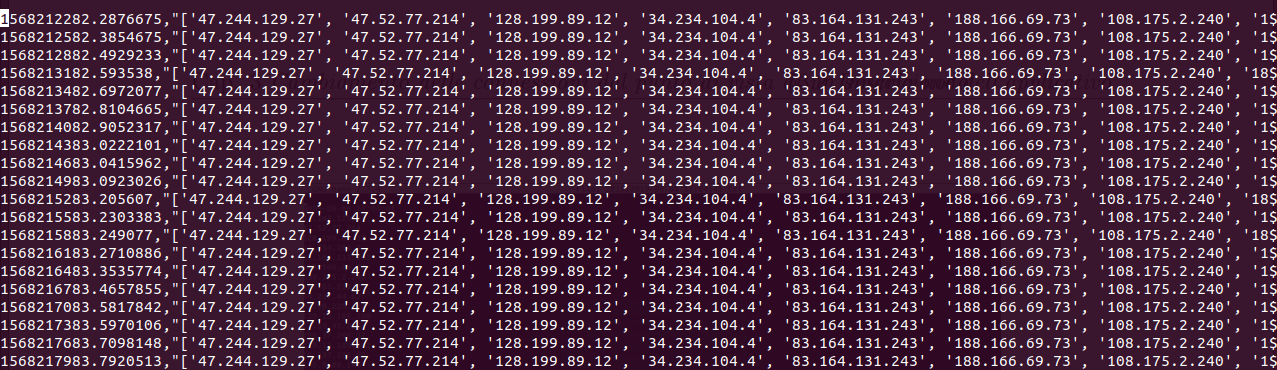
\includegraphics[width=0.755\textwidth]{imgs/dati_csv.png}
   \caption{Esempio dati raccolti.py}
   \end{center}
   \hfill
\end{figure}
dalla monitorizzazione del \textit{full node}, il programma \textit{analisi\_dati\_csv.py} li andr\`a ad elaborare per estrapolarne alcune statistiche. Questo secondo programma dovr\`a essere richiamato con un parametro che indichi il \textit{path} del file di cui siamo interessati. (si veda figura \textit{3.4}).\\
\begin{figure}[htb]
\begin{center}
   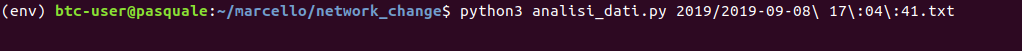
\includegraphics[width=0.755\textwidth]{imgs/analisi_dati.png}
   \caption{Esempio lancio del programma analisi\_dati.py}
   \end{center}
   \hfill
\end{figure}
Alla fine dell'elaborazione del programma saranno create tre cartelle: \textit{risultati\_param1, geolocate\_param1, e intervalli\_param1}.
Nella prima cartella troveremo un file con alcune statitistiche. Alle prime righe saranno identificati il giorno e l'orario in cui la monitorizzazione ha avuto inizio e quello in cui \`e terminata (si veda figura \textit{3.5}).
\begin{figure}[htb]
\begin{center}
   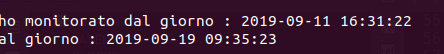
\includegraphics[width=0.755\textwidth]{imgs/tempo.png}
   \caption{Date di inizio e fine monitorizzazionr}
   \end{center}
   \hfill
\end{figure}
Dopo di ch\`e ci sar\`a una lista formata da tre valori: lancio - percentuale - numero di peer connessi(si veda figura \textit{3.6}).
\begin{figure}[htb]
\begin{center}
   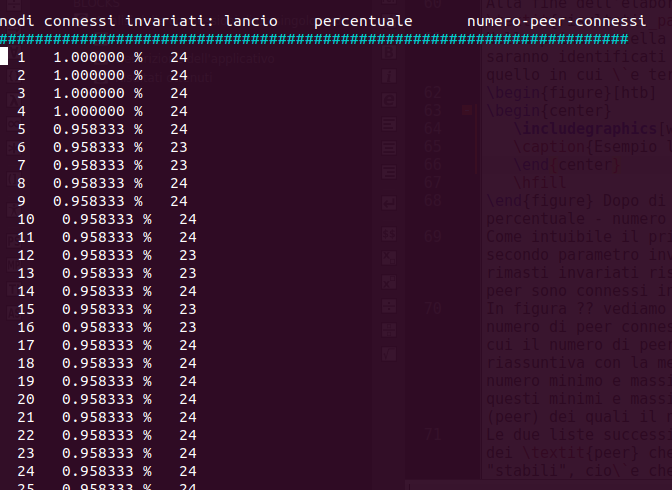
\includegraphics[width=0.755\textwidth]{imgs/lista3.png}
   \caption{Percentuale dei \textit{peer} invariati per ogni lancio}
   \end{center}
   \hfill
\end{figure}
Come intuibile il primo di questi valori indica il numero di lancio considerato, il secondo parametro invece indica quanti peer in percentuale in quel dato lancio sono rimasti invariati rispetto alla prima monitorizzazione, mentre l'ultimo indica quanti peer sono connessi in quel momento.
In figura \textit{3.7} vediamo una lista che indica i lanci in cui si \`e notato il massimo numero di peer connessi (in questo caso 24) e una lista che indica invece i lanci in cui il numero di peer connessi \`e stato minimo (in questo caso 22). Una tabella riassuntiva con la media di peer connessi ad ogni lancio, la relativa varianza, il numero minimo e massimo di peer connessi durante la monitorizzazione, e in quanti lanci questi minimi e massimi si sono verificati. Infine il numero totale di indirizzi IP (peer) dei quali il nostro \textit{full-node} \`e venuto a conoscienza.
Le due liste successive che vediamo sempre in figura contengono invece gli indirizzi dei \textit{peer} che si sono presentati con minor frequenza, e quelli che chiamiamo "stabili", cio\`e che sono sempre rimasti connessi.
\begin{figure}[htb]
\begin{center}
   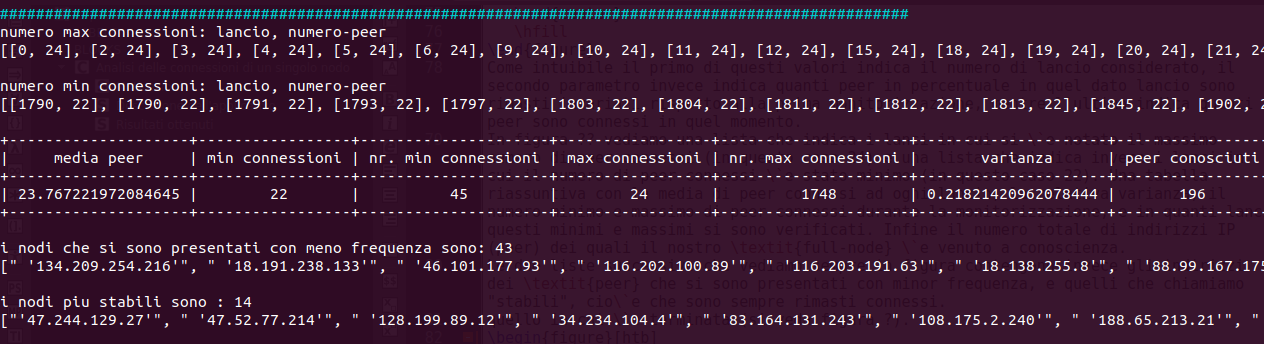
\includegraphics[width=1.000\textwidth]{imgs/tabella1.png}
   \caption{Statistiche sulle connessioni dei \textit{peer}}
   \end{center}
   \hfill
\end{figure}
Il programma mostrer\`a inoltre un rudimentale grafico a barre (figura \textit{3.8}) dove per ogni indirizzo IP ci sar\`a la percentuale di tempo per cui \`e rimasto connesso.
\begin{figure}[htb]
\begin{center}
   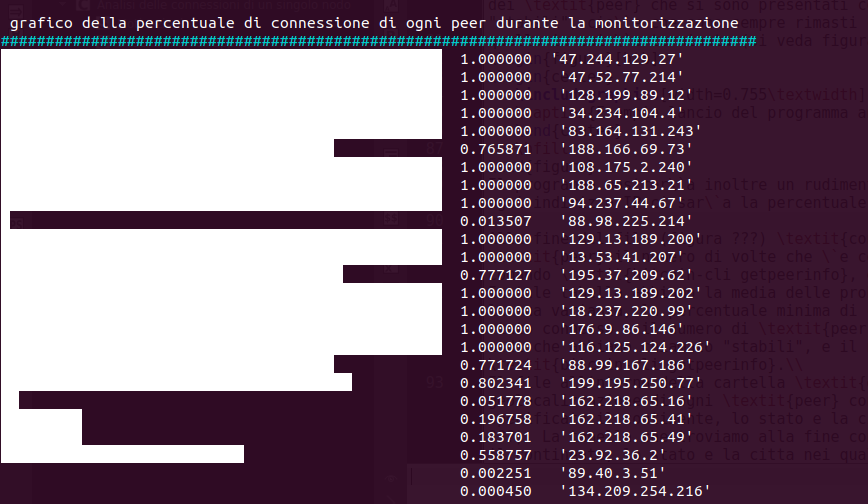
\includegraphics[width=0.755\textwidth]{imgs/grafico.png}
   \caption{Grafico a barre}
   \end{center}
   \hfill
\end{figure}
Alla fine del file (figura \textit{3.9}) \textit{connessioni peer} conterra per ogni \textit{peer} il numero di volte che \`e comparso durante la monitorizzazione del comando \textit{bitcoin-cli getpeerinfo}, e una tabella riassuntiva.
\begin{figure}[htb]
\begin{center}
   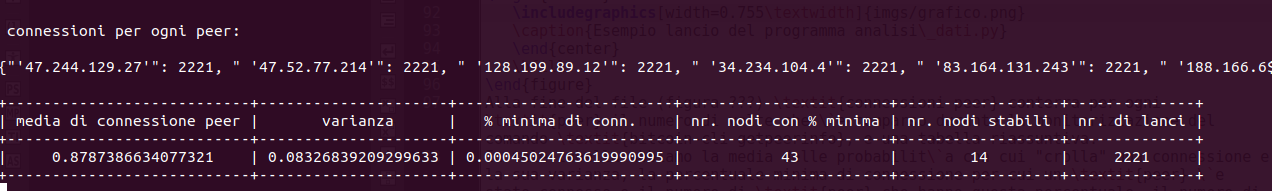
\includegraphics[width=0.755\textwidth]{imgs/tabella2.png}
   \caption{Statistiche sulla percentuale di connessione di ogni peer}
   \end{center}
   \hfill
\end{figure}
In tale tabella abbiamo la media delle probabilit\`a con cui "crolla" una connessione e la sua varianza, la percentuale minima di connessione per cui un \textit{peer} \`e stato connesso e il numero di \textit{peer} che hanno questa percentuale, il numero di nodi che abbiamo chiamato "stabili", e il numero di lanci totali del comando \textit{bitcoin-cli getpeerinfo}.\\
Il file all'nterno della cartella \textit{geolocate\_param1} contiene dati riguardo la geolocalizzazione di ogni \textit{peer} conosciuto. Per ogni indirizzo IP \`e specificato il continente, lo stato e la citt\`a in cui esso si trova (vedi figura \textit{3.10}).
\begin{figure}[htb]
\begin{center}
   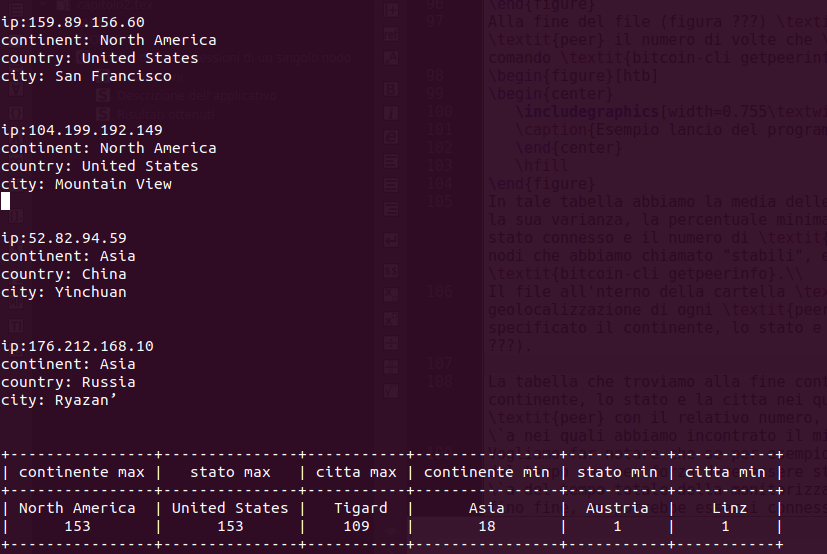
\includegraphics[width=0.755\textwidth]{imgs/geolocate.png}
   \caption{Geolocalizzazione dei \textit{peer}}
   \end{center}
   \hfill
\end{figure}
La tabella che troviamo alla fine contiene alcuni campi importanti tra i quali: il continente, lo stato e la citta nei quali abbiamo incontrato il maggior numero di \textit{peer} con il relativo numero, e analogamente il continente, lo stato e la citt\`a nei quali abbiamo incontrato il minor numero di \textit{peer}.
Vogliamo far notare che se per esempio un \textit{peer} \`e stato connesso per il 50\% del tempo non per forza deve essere stato connesso dall'inizio fino alla fine prima met\`a del tempo totale della monitorizzazione, oppure dall'inizio della seconda met\`a fino fine, ma potrebbe essersi connesso e riconesso pi\`u volte fino a totalizzare la percentuale prima indicata.
Per questo scopo nell'ultima cartella, \textit{intervalli\_param1}, per ogni \textit{peer} viene indicato l'intervallo di tempo in cui questo \`e stato connesso, nel caso quindi di connessioni discontinue, un indirizzo IP sar\`a affiancato da pi\`u intervalli di tempo (si veda figura \textit{3.11}).
\begin{figure}[htb]
\begin{center}
   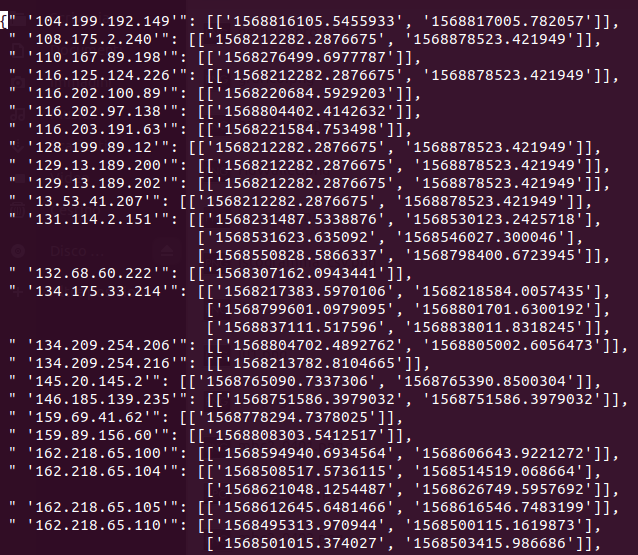
\includegraphics[width=0.755\textwidth]{imgs/intervalli.png}
   \caption{Intervalli di connessione per ogni \textit{peer}}
   \end{center}
   \hfill
\end{figure}




\section{Risultati ottenuti} 
In questo esperimento abbiamo raccolto dati per 10 giorni dal \textit{ 2019-09-11 16:31:22} al \textit{2019-09-19 09:35:23}. Ecco espessi in tabella alcuni risultati che abbiamo ottenuto:

\begin{table}[h!]
    \label{tab:table1}
    \scalebox{1}{
    \begin{tabular}{c|c|c|c|c|c} % <-- Alignments: 1st column left, 2nd middle and 3rd right, with vertical lines in between
      \textbf{Numero Lanci} & \textbf{media peer} & \textbf{varianza} & \textbf{\% nodi invariati} & \textbf{peer conosciuti}\\
      \hline
      2220  & 23.767 &0.218 & 70.1 &196 \\
    \end{tabular}
    }
\end{table}


\begin{table}[h!]
    \label{tab:table1}
    \scalebox{1}{
    \begin{tabular}{c|c|c|c} % <-- Alignments: 1st column left, 2nd middle and 3rd right, with vertical lines in between
      \textbf{max connessioni} & \textbf{nr. max connessioni} & \textbf{min connessioni} & \textbf{nr. min connessioni}\\
      \hline
      24 & 1748 & 22& 43\\
    \end{tabular}
    }
\end{table}
Sappiamo che il protocollo Bitcoin cerca di stabilire per ogni \textit{peer} 24 connessioni con altri nodi per renderlo "ben connesso". Da questi dati vediamo che, per quanto riguarda la nostra analisi, la media delle connessioni si aggira ad un numero molto vicino a 24 e inoltre osservando che la varianza ha un valore basso possiamo dire che in generale il numero di connessioni rimane sempre vicino al 24.\\
Non si \`e mai verificato un caso in cui si \`e superato questo numero di connessioni in un dato istante, ma invece questo \`e stato il massimo valore registrato dal nostro programma, mentre il minimo \`e stato 22, che da appunto conferma, come la varianza, che il numero di connessioni resta sempre "quasi" costante. La maggiorparte delle monitorizzazioni (con precisione 1748/2220) mostrano che il numero di connessioni che Bitcoin cerca di mantenere per ogni nodo \`e esattamente 24.
Il numero di peer per\`o con cui siamo venuti in contatto \`e 196, quindi significa che pi\`u volte delle connessioni sono "crollate" e se ne sono stabilite delle nuove.
Dal grafico a barre riportato dal programma, \`e possibile analizzare la percentuale del tempo totale di connessione per ogni \textit{peer} con il nostro \textit{full-node}. Riportiamo qui solamente i dati che pi\`u ci interessano:\\\\
\begin{table}[h!]
    \label{tab:table1}
    \scalebox{0.8}{
    \begin{tabular}{l|c|c|c|c|r} % <-- Alignments: 1st column left, 2nd middle and 3rd right, with vertical lines in between
      \textbf{media prob. peer} & \textbf{varianza} & \textbf{\% min. connessione} & \textbf{nr. nodi con \% minima} & \textbf{nr. nodi stabili} &\\
      \hline
       0.878 & 0.083 & 0.045\% & 43 & 14 \\
    \end{tabular}
    }
\end{table}
\\non conoscendo come si comporta il protocollo Bitcoin riguardo la topologia della rete, e quindi non sapendo se ci possano essere connessioni con alcuni \textit{peer} pi\`u probabili di altre, abbiamo dato ad ogni \textit{peer} incontrato una probabilit\`a di connettersi al nostro \textit{full-node} a seconda di quante volte \`e stato "incontrato" in passato.
Il primo valore della tabella indica la media di queste probabilit\`a con accanto la relativa varianza, ma questo potrebbe anche non essere quindi un dato che rispecchi effettivamente l'andamento delle cose nel protocollo Bitcoin.
Viene riportato inoltre nella tabella la percentuale minima della connessione di un nodo durante la monitorizzazione. Questa percentuale \`e molto bassa e come vediamo sono ben 43 i nodi che hanno il medesimo valore, questo pu\`o star a significare che c'\`e stato bisogno pi\`u volte di cambiare connessione prima di trovare un nodo pi\`u "stabile". Sono invece 14 i nodi che sono rimasti sempre connessi, e questi potrebbero essere nodi "stabili" della rete, che ci assicurano una connessione all'interno al network Bitcoin e che quindi probabilmente sono necessari.
Per quanto riguarda la geolocalizzazione abbiamo ottenuto:\\
\begin{table}[h!]
    \label{tab:table1}
    \scalebox{0.8}{
    \begin{tabular}{l|c|c|c|c|r} % <-- Alignments: 1st column left, 2nd middle and 3rd right, with vertical lines in between
      \textbf{continente max} & \textbf{stato max} & \textbf{citt\`a max} & \textbf{continente min} & \textbf{stato min} \textbf{citt\`a min}\\
      \hline
      North America & United States & Tigar & Asia & Austria & Linz\\
        153 & 153 & 109 & 18 & 1 & 1\\ 
    \end{tabular}
    }
\end{table}
\\Dove i campi indicano i luoghi e il numero (massimo e minimo ) di peer di cui siamo venuti a conoscenza, rispettivamente per continente, stato e citt\`a.
La maggior parte dei \textit{peer} che abbiamo incontrato, che ricordiamo erano 196, vengono dal nord america, e di questi tutti sono statunitensi, quindi precisamente il 78\% dei \textit{peer} sono americani. Questo potrebbe voler dire che questo \`e il luogo dove la tecnologia si \`e diffusa maggiormente?
In ultimo luogo vogliamo vedere se \`e possibile che un qualche nodo che si disconnette dal nostro \textit{full-node} sia propenso, o almeno ci sia qualche probabili\`a che possa ristabilire una connessione.
Come mostato dai dati ricavati dal nostro programma di analisi, vediamo che questa situazione capita non di rado, mostriamo gli intervalli di tempo (rappresentiamo i timestamp) di alcuni peer per cui si \`e vefiricato questo fatto:

\begin{table}[h!]
    \label{tab:table1}
    \scalebox{0.7}{
    \begin{tabular}{c|c|c} % <-- Alignments: 1st column left, 2nd middle and 3rd right, with vertical lines in between
      \textbf{131.114.2.151} & \textbf{162.218.65.241} & \textbf{23.92.36.28} \\
      \hline
      (1568231487.5338876, 1568530123.2425718) & (1568540025.947396, 1568543326.6773708) & (1568584437.7690363, 1568586538.3642185)\\ 
        (1568531623.635092, 1568546027.300046) & (1568668761.6218576, 1568668761.6218576) & (1568587138.5555046, 1568595540.8496878)\\
         (1568550828.5866337, 1568798400.6723945) & (1568669961.9677079, 1568673563.005906)\\ 
    \end{tabular}
    }
\end{table}
 
 
  












\chapter{Conclusioni e sviluppi futuri}
In questa tesi si \`e fatta una panoramica di tutto ci\`o che riguarda l'ecosistema Bitcoin, con particolare attenzione a ci\`o che concerne la rete peer-to-peer che \`e una parte di importanza centrale di tale tecnologia. Succissivamente \`e stato presentato un applicativo in grado di fornire informazioni riguardo una piccola parte della topologia della rete Bitcoin, cio\`e quella riguardante le connessioni di un singolo \textit{full node} con i suoi \textit{peers}. \\
Siamo quindi cosi riusciti a fare un 'analisi pi\`u o meno accurata per quanto riguarda le connessioni di un singolo nodo, e i risultati di tale analisi sono stati evidenziati nel capitolo 3.
Questo lavoro avrebbe come obiettivo per\`o quello di riuscire a monitorare ogni nodo della rete, per poter inferire le connessioni non di un solo \textit{full node}, ma di ogni partecipante della rete, per questo deve essere considerato soltanto come un passo intermedio per il raggiungimento di un obiettivo pi\`u ambizioso.

\chapter*{Appendice A}

\subsubsection{codice latex di questa tesi:}


\subsubsection{app messagistica:}


\subsubsection{app usata per i test:}




% ELENCO DELLE FIGURE (OPZIONALE)
\addcontentsline{toc}{chapter}{Elenco delle figure}
\listoffigures


% BIBLIOGRAFIA
% \addcontentsline{toc}{chapter}{Bibliografia}

\bibliography{biblio} 
\bibliographystyle{plain}

\end{document}
